\documentclass[11pt]{article}
\usepackage[a4paper,margin=2.5cm]{geometry}
\usepackage[T1]{fontenc}
\usepackage{amsmath,amssymb,graphicx,booktabs}
\usepackage[numbers,super,sort&compress]{natbib}
\usepackage[hidelinks]{hyperref}
\usepackage{xcolor}
\usepackage{placeins}
\usepackage[labelsep=period]{caption}
\usepackage{pgfplots}
\usepgfplotslibrary{groupplots}
\usetikzlibrary{shapes.geometric}
\pgfplotsset{compat=1.16}
\definecolor{cA}{HTML}{24588F}\definecolor{cB}{HTML}{C4572E}\definecolor{cC}{HTML}{A8A79F}\definecolor{cD}{HTML}{6B4C9A}
\pgfplotsset{pub/.style={axis lines=left,axis line style={-,line width=0.4pt,black!75},tick style={line width=0.4pt,black!75},tick align=outside,major tick length=2pt,tick label style={font=\sffamily\scriptsize,/pgf/number format/assume math mode=true},every axis label/.append style={font=\sffamily\footnotesize},log ticks with fixed point,title style={font=\sffamily\footnotesize,anchor=south west,at={(0,1.03)},align=left},legend style={draw=none,fill=none,font=\sffamily\scriptsize,cells={anchor=west}},every axis plot/.append style={line width=0.9pt},clip=false,xlabel near ticks,ylabel near ticks}}

\newcommand{\figasym}{%
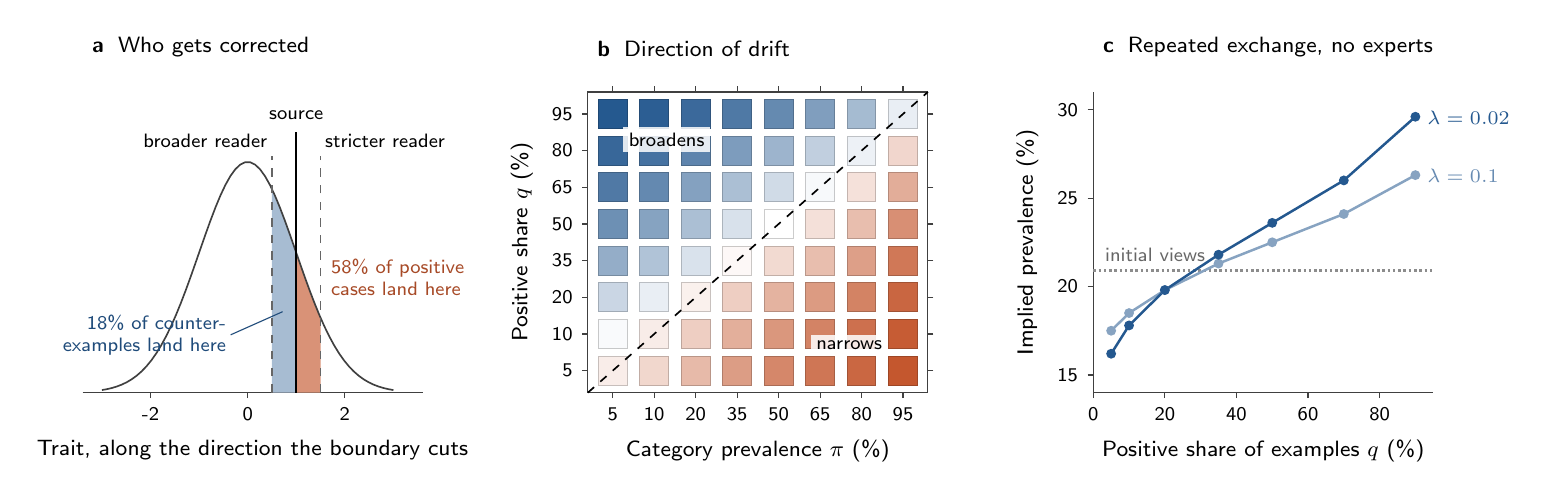
\begin{tikzpicture}[font=\sffamily\footnotesize]
\begin{groupplot}[pub,group style={group size=3 by 1,horizontal sep=2.1cm},width=5.9cm,height=5.4cm]
\nextgroupplot[title={\textbf{a}\hspace{0.6em}Who gets corrected},xlabel={Trait, along the direction the boundary cuts},axis y line=none,xmin=-3,xmax=3,ymin=0,ymax=0.52,xtick={-2,0,2},xmin=-3.4,xmax=3.6]
\addplot[draw=none,fill=cA!40,domain=0.5:1,samples=12,line width=0pt] {exp(-x^2/2)/2.5066} \closedcycle;
\addplot[draw=none,fill=cB!65,domain=1:1.5,samples=12,line width=0pt] {exp(-x^2/2)/2.5066} \closedcycle;
\addplot[black!75,domain=-3:3,samples=60,line width=0.6pt] {exp(-x^2/2)/2.5066};
\draw[black,line width=0.9pt] (axis cs:1,0) -- (axis cs:1,0.45);
\draw[black!60,dashed,line width=0.5pt] (axis cs:0.5,0) -- (axis cs:0.5,0.41);
\draw[black!60,dashed,line width=0.5pt] (axis cs:1.5,0) -- (axis cs:1.5,0.41);
\node[font=\sffamily\scriptsize,text=black,anchor=south,inner sep=1.5pt] at (axis cs:1,0.465) {source};
\node[font=\sffamily\scriptsize,text=black,anchor=south east,inner sep=1.5pt] at (axis cs:0.5,0.415) {broader reader};
\node[font=\sffamily\scriptsize,text=black,anchor=south west,inner sep=1.5pt] at (axis cs:1.5,0.415) {stricter reader};
\node[font=\sffamily\scriptsize,text=cB!85!black,anchor=west,inner sep=1.5pt,align=left] at (axis cs:1.62,0.2) {58\% of positive\\cases land here};
\node[font=\sffamily\scriptsize,text=cA!85!black,anchor=east,inner sep=1.5pt,align=right] at (axis cs:-0.35,0.1) {18\% of counter-\\examples land here};
\draw[cA!85!black,line width=0.4pt] (axis cs:-0.35,0.1) -- (axis cs:0.72,0.14);
\nextgroupplot[title={\textbf{b}\hspace{0.6em}Direction of drift},axis lines=box,xlabel={Category prevalence $\pi$ (\%)},ylabel={Positive share $q$ (\%)},clip marker paths=true,xtick={1,...,8},ytick={1,...,8},xticklabels={5,10,20,35,50,65,80,95},yticklabels={5,10,20,35,50,65,80,95},xmin=0.4,xmax=8.6,ymin=0.4,ymax=8.6,tick align=outside,colormap={dv}{color=(cB) color=(white) color=(cA)},point meta min=-0.0991,point meta max=0.0991]
\addplot[scatter,only marks,mark=square*,mark size=5.2pt,point meta=explicit,line width=0pt] coordinates {(1,1) [-0.0103] (2,1) [-0.0237] (3,1) [-0.0407] (4,1) [-0.058] (5,1) [-0.0705] (6,1) [-0.0807] (7,1) [-0.0896] (8,1) [-0.0991] (1,2) [0.00293] (2,2) [-0.0109] (3,2) [-0.0287] (4,2) [-0.0472] (5,2) [-0.0614] (6,2) [-0.0731] (7,2) [-0.0841] (8,2) [-0.0962] (1,3) [0.0242] (2,3) [0.0102] (3,3) [-0.00839] (4,3) [-0.0287] (5,3) [-0.0448] (6,3) [-0.0591] (7,3) [-0.0733] (8,3) [-0.0903] (1,4) [0.0486] (2,4) [0.0356] (3,4) [0.0172] (4,4) [-0.00387] (5,4) [-0.0217] (6,4) [-0.0385] (7,4) [-0.0565] (8,4) [-0.0795] (1,5) [0.0662] (2,5) [0.0549] (3,5) [0.038] (4,5) [0.0179] (5,5) [0.000153] (6,5) [-0.018] (7,5) [-0.0382] (8,5) [-0.066] (1,6) [0.0795] (2,6) [0.0701] (3,6) [0.0559] (4,6) [0.0382] (5,6) [0.0214] (6,6) [0.00354] (7,6) [-0.0174] (8,6) [-0.0483] (1,7) [0.0902] (2,7) [0.0836] (3,7) [0.0728] (4,7) [0.0587] (5,7) [0.0443] (6,7) [0.0283] (7,7) [0.00817] (8,7) [-0.0239] (1,8) [0.0989] (2,8) [0.0954] (3,8) [0.089] (4,8) [0.0798] (5,8) [0.0698] (6,8) [0.0576] (7,8) [0.0406] (8,8) [0.0101]};
\draw[black,dashed,line width=0.6pt] (axis cs:0.4,0.4) -- (axis cs:8.6,8.6);
\node[font=\sffamily\scriptsize,fill=white,fill opacity=0.85,text opacity=1,inner sep=2pt] at (axis cs:2.3,7.3) {broadens};
\node[font=\sffamily\scriptsize,fill=white,fill opacity=0.85,text opacity=1,inner sep=2pt] at (axis cs:6.7,1.7) {narrows};
\nextgroupplot[title={\textbf{c}\hspace{0.6em}Repeated exchange, no experts},xlabel={Positive share of examples $q$ (\%)},ylabel={Implied prevalence (\%)},xmin=0,xmax=95,ymin=14,ymax=31]
\addplot[black!45,densely dotted] coordinates {(0,20.9) (95,20.9)};
\addplot[cA!55,mark=*,mark size=1.3pt] coordinates {(5,17.5) (10,18.5) (20,19.8) (35,21.3) (50,22.5) (70,24.1) (90,26.3)};
\addplot[cA,mark=*,mark size=1.3pt] coordinates {(5,16.2) (10,17.8) (20,19.8) (35,21.8) (50,23.6) (70,26) (90,29.6)};
\node[font=\sffamily\scriptsize,text=cA,anchor=west,inner sep=1.5pt] at (axis cs:92,29.55954973863576) {$\lambda=0.02$};
\node[font=\sffamily\scriptsize,text=cA!70,anchor=west,inner sep=1.5pt] at (axis cs:92,26.27167467397291) {$\lambda=0.1$};
\node[font=\sffamily\scriptsize,text=black!60,anchor=south west,inner sep=1.5pt] at (axis cs:2,21.134628723162795) {initial views};
\end{groupplot}
\end{tikzpicture}}

\newcommand{\figmech}{%
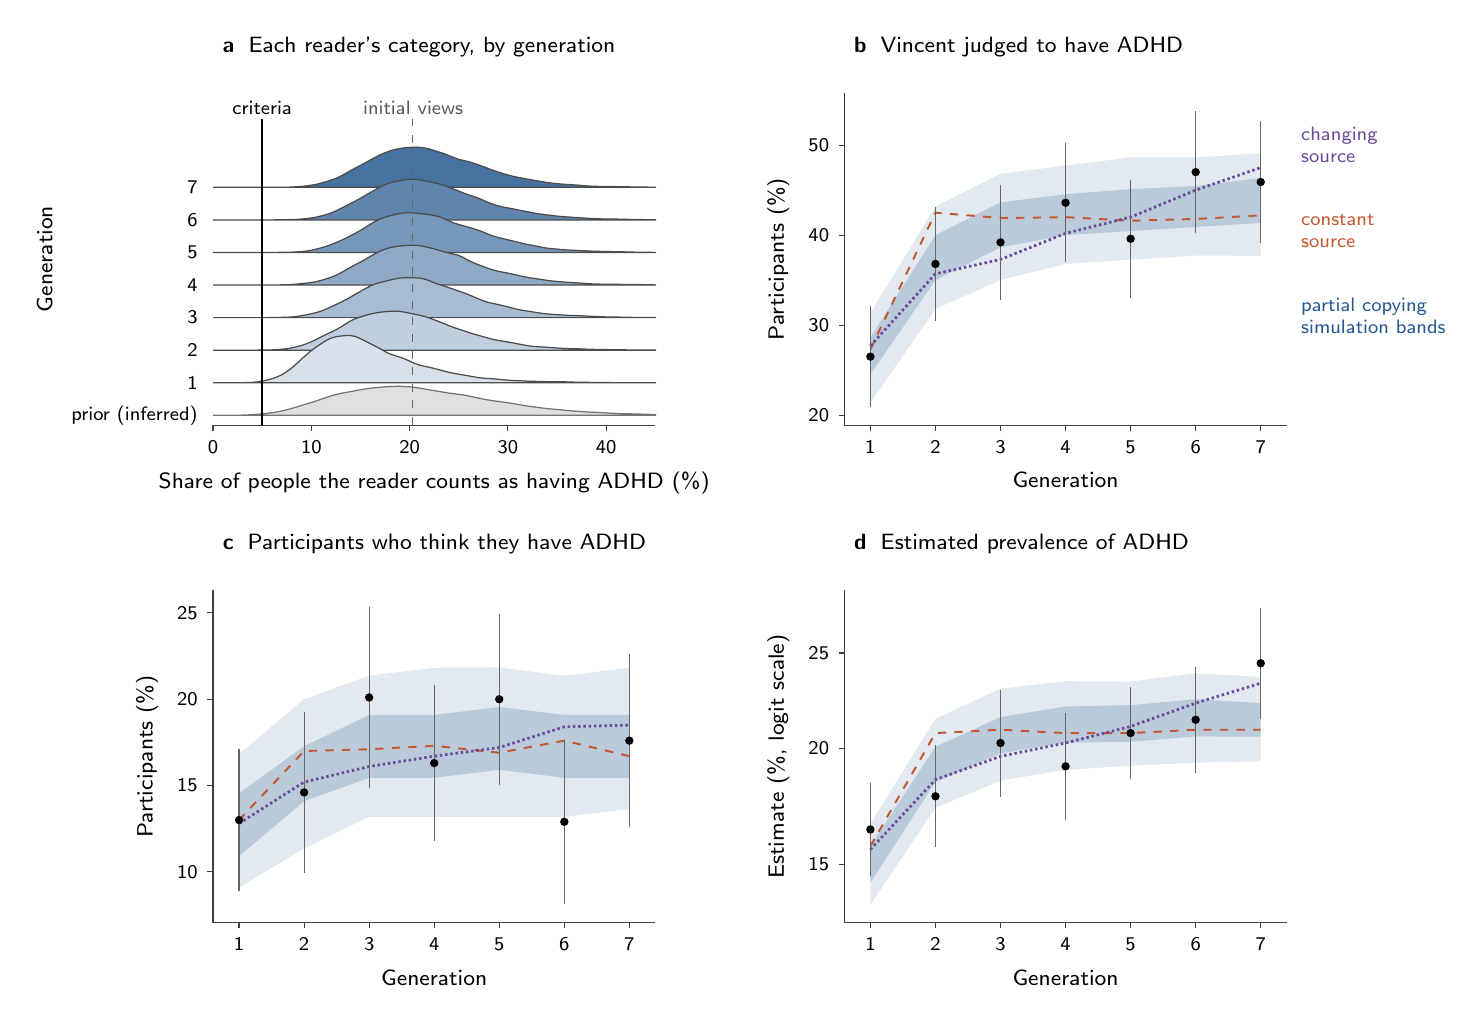
\begin{tikzpicture}[font=\sffamily\footnotesize]
\begin{groupplot}[pub,group style={group size=2 by 2,horizontal sep=2.4cm,vertical sep=2.1cm},width=7.2cm,height=5.8cm]
\nextgroupplot[title={\textbf{a}\hspace{0.6em}Each reader's category, by generation},xlabel={Share of people the reader counts as having ADHD (\%)},xmin=0,xmax=45,ymin=-0.3,ymax=9.9,ytick={0,1,...,7},yticklabels={prior (inferred),1,2,3,4,5,6,7},axis y line*=left,y axis line style={draw=none},ytick style={draw=none},ylabel={Generation},clip=false]
\addplot[fill=cA!84!white,draw=black!70,line width=0.45pt] coordinates {(0,7) (0.0,7.000) (0.5,7.000) (1.0,7.000) (1.5,7.000) (2.0,7.000) (2.5,7.000) (3.0,7.000) (3.5,7.000) (4.0,7.000) (4.5,7.000) (5.0,7.000) (5.5,7.000) (6.0,7.001) (6.5,7.001) (7.0,7.002) (7.5,7.004) (8.0,7.009) (8.5,7.018) (9.0,7.030) (9.5,7.046) (10.0,7.066) (10.5,7.093) (11.0,7.130) (11.5,7.173) (12.0,7.222) (12.5,7.276) (13.0,7.344) (13.5,7.428) (14.0,7.517) (14.5,7.598) (15.0,7.674) (15.5,7.755) (16.0,7.841) (16.5,7.924) (17.0,7.998) (17.5,8.063) (18.0,8.118) (18.5,8.163) (19.0,8.194) (19.5,8.215) (20.0,8.227) (20.5,8.231) (21.0,8.228) (21.5,8.212) (22.0,8.179) (22.5,8.132) (23.0,8.084) (23.5,8.036) (24.0,7.977) (24.5,7.912) (25.0,7.860) (25.5,7.825) (26.0,7.789) (26.5,7.743) (27.0,7.691) (27.5,7.636) (28.0,7.578) (28.5,7.523) (29.0,7.473) (29.5,7.424) (30.0,7.379) (30.5,7.341) (31.0,7.310) (31.5,7.280) (32.0,7.252) (32.5,7.226) (33.0,7.200) (33.5,7.173) (34.0,7.149) (34.5,7.130) (35.0,7.114) (35.5,7.100) (36.0,7.090) (36.5,7.081) (37.0,7.070) (37.5,7.057) (38.0,7.045) (38.5,7.037) (39.0,7.031) (39.5,7.028) (40.0,7.027) (40.5,7.025) (41.0,7.023) (41.5,7.021) (42.0,7.018) (42.5,7.014) (43.0,7.011) (43.5,7.009) (44.0,7.008) (44.5,7.006) (45.0,7.005) (45,7)} -- cycle;
\addplot[fill=cA!73!white,draw=black!70,line width=0.45pt] coordinates {(0,6) (0.0,6.000) (0.5,6.000) (1.0,6.000) (1.5,6.000) (2.0,6.000) (2.5,6.000) (3.0,6.000) (3.5,6.000) (4.0,6.000) (4.5,6.000) (5.0,6.000) (5.5,6.000) (6.0,6.001) (6.5,6.002) (7.0,6.004) (7.5,6.007) (8.0,6.011) (8.5,6.017) (9.0,6.027) (9.5,6.041) (10.0,6.060) (10.5,6.086) (11.0,6.121) (11.5,6.162) (12.0,6.212) (12.5,6.275) (13.0,6.350) (13.5,6.430) (14.0,6.506) (14.5,6.582) (15.0,6.665) (15.5,6.753) (16.0,6.841) (16.5,6.928) (17.0,7.012) (17.5,7.085) (18.0,7.139) (18.5,7.176) (19.0,7.209) (19.5,7.236) (20.0,7.249) (20.5,7.247) (21.0,7.231) (21.5,7.205) (22.0,7.175) (22.5,7.143) (23.0,7.107) (23.5,7.061) (24.0,7.004) (24.5,6.945) (25.0,6.886) (25.5,6.825) (26.0,6.771) (26.5,6.723) (27.0,6.668) (27.5,6.603) (28.0,6.537) (28.5,6.479) (29.0,6.432) (29.5,6.396) (30.0,6.368) (30.5,6.341) (31.0,6.311) (31.5,6.280) (32.0,6.250) (32.5,6.220) (33.0,6.193) (33.5,6.172) (34.0,6.154) (34.5,6.136) (35.0,6.118) (35.5,6.104) (36.0,6.093) (36.5,6.082) (37.0,6.072) (37.5,6.062) (38.0,6.053) (38.5,6.043) (39.0,6.036) (39.5,6.032) (40.0,6.030) (40.5,6.028) (41.0,6.026) (41.5,6.022) (42.0,6.019) (42.5,6.016) (43.0,6.013) (43.5,6.010) (44.0,6.009) (44.5,6.008) (45.0,6.005) (45,6)} -- cycle;
\addplot[fill=cA!62!white,draw=black!70,line width=0.45pt] coordinates {(0,5) (0.0,5.000) (0.5,5.000) (1.0,5.000) (1.5,5.000) (2.0,5.000) (2.5,5.000) (3.0,5.000) (3.5,5.000) (4.0,5.000) (4.5,5.000) (5.0,5.001) (5.5,5.001) (6.0,5.002) (6.5,5.003) (7.0,5.005) (7.5,5.007) (8.0,5.011) (8.5,5.018) (9.0,5.028) (9.5,5.043) (10.0,5.069) (10.5,5.103) (11.0,5.142) (11.5,5.187) (12.0,5.241) (12.5,5.302) (13.0,5.368) (13.5,5.438) (14.0,5.515) (14.5,5.596) (15.0,5.681) (15.5,5.772) (16.0,5.867) (16.5,5.957) (17.0,6.030) (17.5,6.085) (18.0,6.128) (18.5,6.166) (19.0,6.197) (19.5,6.217) (20.0,6.221) (20.5,6.212) (21.0,6.195) (21.5,6.178) (22.0,6.160) (22.5,6.136) (23.0,6.099) (23.5,6.042) (24.0,5.970) (24.5,5.906) (25.0,5.860) (25.5,5.819) (26.0,5.776) (26.5,5.731) (27.0,5.682) (27.5,5.625) (28.0,5.561) (28.5,5.505) (29.0,5.462) (29.5,5.425) (30.0,5.390) (30.5,5.355) (31.0,5.317) (31.5,5.278) (32.0,5.246) (32.5,5.220) (33.0,5.189) (33.5,5.157) (34.0,5.133) (34.5,5.117) (35.0,5.104) (35.5,5.089) (36.0,5.078) (36.5,5.071) (37.0,5.064) (37.5,5.057) (38.0,5.049) (38.5,5.042) (39.0,5.038) (39.5,5.033) (40.0,5.029) (40.5,5.027) (41.0,5.025) (41.5,5.022) (42.0,5.018) (42.5,5.014) (43.0,5.010) (43.5,5.008) (44.0,5.006) (44.5,5.004) (45.0,5.003) (45,5)} -- cycle;
\addplot[fill=cA!51!white,draw=black!70,line width=0.45pt] coordinates {(0,4) (0.0,4.000) (0.5,4.000) (1.0,4.000) (1.5,4.000) (2.0,4.000) (2.5,4.000) (3.0,4.000) (3.5,4.000) (4.0,4.000) (4.5,4.000) (5.0,4.000) (5.5,4.000) (6.0,4.001) (6.5,4.003) (7.0,4.007) (7.5,4.012) (8.0,4.019) (8.5,4.029) (9.0,4.043) (9.5,4.059) (10.0,4.079) (10.5,4.106) (11.0,4.143) (11.5,4.188) (12.0,4.238) (12.5,4.298) (13.0,4.374) (13.5,4.463) (14.0,4.550) (14.5,4.629) (15.0,4.707) (15.5,4.792) (16.0,4.880) (16.5,4.966) (17.0,5.042) (17.5,5.103) (18.0,5.148) (18.5,5.178) (19.0,5.198) (19.5,5.211) (20.0,5.220) (20.5,5.221) (21.0,5.210) (21.5,5.185) (22.0,5.150) (22.5,5.110) (23.0,5.065) (23.5,5.020) (24.0,4.983) (24.5,4.953) (25.0,4.910) (25.5,4.839) (26.0,4.757) (26.5,4.685) (27.0,4.625) (27.5,4.568) (28.0,4.511) (28.5,4.463) (29.0,4.425) (29.5,4.395) (30.0,4.366) (30.5,4.335) (31.0,4.299) (31.5,4.264) (32.0,4.236) (32.5,4.213) (33.0,4.190) (33.5,4.167) (34.0,4.144) (34.5,4.125) (35.0,4.111) (35.5,4.099) (36.0,4.087) (36.5,4.076) (37.0,4.067) (37.5,4.058) (38.0,4.047) (38.5,4.037) (39.0,4.030) (39.5,4.028) (40.0,4.028) (40.5,4.028) (41.0,4.025) (41.5,4.021) (42.0,4.018) (42.5,4.017) (43.0,4.016) (43.5,4.014) (44.0,4.011) (44.5,4.008) (45.0,4.005) (45,4)} -- cycle;
\addplot[fill=cA!40!white,draw=black!70,line width=0.45pt] coordinates {(0,3) (0.0,3.000) (0.5,3.000) (1.0,3.000) (1.5,3.000) (2.0,3.000) (2.5,3.000) (3.0,3.000) (3.5,3.000) (4.0,3.000) (4.5,3.000) (5.0,3.000) (5.5,3.000) (6.0,3.002) (6.5,3.004) (7.0,3.008) (7.5,3.012) (8.0,3.021) (8.5,3.036) (9.0,3.059) (9.5,3.087) (10.0,3.118) (10.5,3.156) (11.0,3.202) (11.5,3.261) (12.0,3.330) (12.5,3.401) (13.0,3.471) (13.5,3.547) (14.0,3.633) (14.5,3.721) (15.0,3.807) (15.5,3.892) (16.0,3.971) (16.5,4.033) (17.0,4.078) (17.5,4.115) (18.0,4.153) (18.5,4.189) (19.0,4.214) (19.5,4.224) (20.0,4.224) (20.5,4.222) (21.0,4.216) (21.5,4.187) (22.0,4.132) (22.5,4.070) (23.0,4.016) (23.5,3.969) (24.0,3.920) (24.5,3.868) (25.0,3.816) (25.5,3.763) (26.0,3.704) (26.5,3.641) (27.0,3.576) (27.5,3.516) (28.0,3.468) (28.5,3.434) (29.0,3.402) (29.5,3.367) (30.0,3.330) (30.5,3.290) (31.0,3.252) (31.5,3.223) (32.0,3.200) (32.5,3.177) (33.0,3.152) (33.5,3.130) (34.0,3.114) (34.5,3.102) (35.0,3.092) (35.5,3.081) (36.0,3.071) (36.5,3.066) (37.0,3.062) (37.5,3.056) (38.0,3.048) (38.5,3.040) (39.0,3.033) (39.5,3.028) (40.0,3.022) (40.5,3.019) (41.0,3.017) (41.5,3.015) (42.0,3.012) (42.5,3.008) (43.0,3.006) (43.5,3.005) (44.0,3.006) (44.5,3.007) (45.0,3.007) (45,3)} -- cycle;
\addplot[fill=cA!29!white,draw=black!70,line width=0.45pt] coordinates {(0,2) (0.0,2.000) (0.5,2.000) (1.0,2.000) (1.5,2.000) (2.0,2.000) (2.5,2.000) (3.0,2.000) (3.5,2.000) (4.0,2.001) (4.5,2.002) (5.0,2.003) (5.5,2.006) (6.0,2.010) (6.5,2.017) (7.0,2.029) (7.5,2.046) (8.0,2.071) (8.5,2.103) (9.0,2.146) (9.5,2.197) (10.0,2.258) (10.5,2.329) (11.0,2.408) (11.5,2.484) (12.0,2.553) (12.5,2.625) (13.0,2.711) (13.5,2.809) (14.0,2.900) (14.5,2.970) (15.0,3.021) (15.5,3.067) (16.0,3.109) (16.5,3.141) (17.0,3.165) (17.5,3.183) (18.0,3.195) (18.5,3.199) (19.0,3.190) (19.5,3.167) (20.0,3.137) (20.5,3.107) (21.0,3.075) (21.5,3.037) (22.0,2.991) (22.5,2.934) (23.0,2.875) (23.5,2.816) (24.0,2.755) (24.5,2.697) (25.0,2.646) (25.5,2.596) (26.0,2.545) (26.5,2.497) (27.0,2.456) (27.5,2.414) (28.0,2.368) (28.5,2.329) (29.0,2.300) (29.5,2.277) (30.0,2.252) (30.5,2.225) (31.0,2.195) (31.5,2.166) (32.0,2.140) (32.5,2.119) (33.0,2.107) (33.5,2.099) (34.0,2.091) (34.5,2.079) (35.0,2.066) (35.5,2.056) (36.0,2.049) (36.5,2.046) (37.0,2.043) (37.5,2.038) (38.0,2.032) (38.5,2.027) (39.0,2.023) (39.5,2.020) (40.0,2.018) (40.5,2.016) (41.0,2.014) (41.5,2.012) (42.0,2.010) (42.5,2.007) (43.0,2.004) (43.5,2.003) (44.0,2.002) (44.5,2.003) (45.0,2.003) (45,2)} -- cycle;
\addplot[fill=cA!18!white,draw=black!70,line width=0.45pt] coordinates {(0,1) (0.0,1.000) (0.5,1.000) (1.0,1.000) (1.5,1.000) (2.0,1.000) (2.5,1.001) (3.0,1.002) (3.5,1.005) (4.0,1.012) (4.5,1.026) (5.0,1.050) (5.5,1.082) (6.0,1.124) (6.5,1.177) (7.0,1.246) (7.5,1.338) (8.0,1.452) (8.5,1.584) (9.0,1.723) (9.5,1.860) (10.0,1.987) (10.5,2.099) (11.0,2.200) (11.5,2.294) (12.0,2.370) (12.5,2.414) (13.0,2.435) (13.5,2.449) (14.0,2.450) (14.5,2.419) (15.0,2.355) (15.5,2.276) (16.0,2.200) (16.5,2.127) (17.0,2.046) (17.5,1.959) (18.0,1.885) (18.5,1.833) (19.0,1.788) (19.5,1.732) (20.0,1.664) (20.5,1.597) (21.0,1.544) (21.5,1.507) (22.0,1.475) (22.5,1.438) (23.0,1.397) (23.5,1.357) (24.0,1.320) (24.5,1.289) (25.0,1.262) (25.5,1.237) (26.0,1.211) (26.5,1.184) (27.0,1.158) (27.5,1.140) (28.0,1.130) (28.5,1.121) (29.0,1.108) (29.5,1.093) (30.0,1.080) (30.5,1.069) (31.0,1.062) (31.5,1.056) (32.0,1.049) (32.5,1.045) (33.0,1.042) (33.5,1.038) (34.0,1.033) (34.5,1.030) (35.0,1.030) (35.5,1.030) (36.0,1.027) (36.5,1.022) (37.0,1.017) (37.5,1.015) (38.0,1.013) (38.5,1.011) (39.0,1.009) (39.5,1.007) (40.0,1.005) (40.5,1.004) (41.0,1.003) (41.5,1.003) (42.0,1.003) (42.5,1.003) (43.0,1.003) (43.5,1.003) (44.0,1.003) (44.5,1.002) (45.0,1.002) (45,1)} -- cycle;
\addplot[fill=black!12,draw=black!55,line width=0.45pt] coordinates {(0,0) (0.0,0.000) (0.5,0.000) (1.0,0.000) (1.5,0.000) (2.0,0.001) (2.5,0.003) (3.0,0.007) (3.5,0.012) (4.0,0.021) (4.5,0.031) (5.0,0.045) (5.5,0.061) (6.0,0.080) (6.5,0.103) (7.0,0.133) (7.5,0.169) (8.0,0.211) (8.5,0.256) (9.0,0.303) (9.5,0.348) (10.0,0.394) (10.5,0.442) (11.0,0.493) (11.5,0.546) (12.0,0.596) (12.5,0.638) (13.0,0.672) (13.5,0.700) (14.0,0.728) (14.5,0.759) (15.0,0.788) (15.5,0.812) (16.0,0.831) (16.5,0.848) (17.0,0.863) (17.5,0.875) (18.0,0.884) (18.5,0.889) (19.0,0.890) (19.5,0.886) (20.0,0.876) (20.5,0.859) (21.0,0.836) (21.5,0.810) (22.0,0.783) (22.5,0.758) (23.0,0.733) (23.5,0.707) (24.0,0.683) (24.5,0.662) (25.0,0.643) (25.5,0.622) (26.0,0.595) (26.5,0.563) (27.0,0.530) (27.5,0.498) (28.0,0.470) (28.5,0.447) (29.0,0.427) (29.5,0.407) (30.0,0.386) (30.5,0.362) (31.0,0.336) (31.5,0.310) (32.0,0.286) (32.5,0.263) (33.0,0.242) (33.5,0.224) (34.0,0.207) (34.5,0.193) (35.0,0.180) (35.5,0.166) (36.0,0.151) (36.5,0.137) (37.0,0.124) (37.5,0.114) (38.0,0.105) (38.5,0.097) (39.0,0.090) (39.5,0.082) (40.0,0.074) (40.5,0.065) (41.0,0.058) (41.5,0.052) (42.0,0.048) (42.5,0.045) (43.0,0.041) (43.5,0.037) (44.0,0.033) (44.5,0.028) (45.0,0.024) (45,0)} -- cycle;
\draw[black,line width=0.7pt] (axis cs:5,-0.3) -- (axis cs:5,9.1);
\draw[black!60,dashed,line width=0.6pt] (axis cs:20.3,-0.3) -- (axis cs:20.3,9.1);
\node[font=\sffamily\scriptsize,text=black,anchor=south,inner sep=1.5pt] at (axis cs:5,9.1) {criteria};
\node[font=\sffamily\scriptsize,text=black!65,anchor=south,inner sep=1.5pt] at (axis cs:20.349471935114583,9.1) {initial views};
\nextgroupplot[title={\textbf{b}\hspace{0.6em}Vincent judged to have ADHD},ylabel={Participants (\%)},xlabel={Generation},xtick={1,...,7},xmin=0.6,xmax=7.4,ymin=18.9,ymax=55.8]
\addplot[fill=cA!13,draw=none,line width=0pt] coordinates {(1,31.36) (2,43.18) (3,46.82) (4,47.73) (5,48.64) (6,48.64) (7,49.09) (7,37.7) (6,37.73) (5,37.27) (4,36.8) (3,35) (2,31.82) (1,21.36)} -- cycle;
\addplot[fill=cA!32,draw=none,line width=0pt] coordinates {(1,28.64) (2,40) (3,43.64) (4,44.55) (5,45.11) (6,45.45) (7,46.36) (7,41.36) (6,40.91) (5,40.45) (4,40) (3,38.64) (2,35) (1,24.55)} -- cycle;
\addplot[cB,dashed,line width=0.7pt] coordinates {(1,27.3) (2,42.5) (3,41.9) (4,42) (5,41.6) (6,41.8) (7,42.2)};
\addplot[cD,densely dotted,line width=1pt] coordinates {(1,27.7) (2,35.7) (3,37.3) (4,40.2) (5,42) (6,45) (7,47.5)};
\addplot[black,only marks,mark=*,mark size=1.3pt,line width=0.4pt,error bars/.cd,y dir=both,y explicit,error bar style={line width=0.4pt,black!60},error mark=none] coordinates {(1,26.5) +- (0,5.62) (2,36.8) +- (0,6.37) (3,39.2) +- (0,6.4) (4,43.6) +- (0,6.6) (5,39.6) +- (0,6.55) (6,47) +- (0,6.76) (7,45.9) +- (0,6.81)};
\node[font=\sffamily\scriptsize,text=cA,anchor=west,inner sep=1.5pt,align=left] at (axis cs:7.55,31) {partial copying\\simulation bands};
\node[font=\sffamily\scriptsize,text=cB,anchor=west,inner sep=1.5pt,align=left] at (axis cs:7.55,40.5) {constant\\source};
\node[font=\sffamily\scriptsize,text=cD,anchor=west,inner sep=1.5pt,align=left] at (axis cs:7.55,50) {changing\\source};
\nextgroupplot[title={\textbf{c}\hspace{0.6em}Participants who think they have ADHD},ylabel={Participants (\%)},xlabel={Generation},xtick={1,...,7},xmin=0.6,xmax=7.4,ymin=7.06,ymax=26.3]
\addplot[fill=cA!13,draw=none,line width=0pt] coordinates {(1,16.82) (2,20) (3,21.36) (4,21.82) (5,21.84) (6,21.36) (7,21.82) (7,13.64) (6,13.18) (5,13.18) (4,13.18) (3,13.18) (2,11.36) (1,9.091)} -- cycle;
\addplot[fill=cA!32,draw=none,line width=0pt] coordinates {(1,14.55) (2,17.27) (3,19.09) (4,19.09) (5,19.55) (6,19.09) (7,19.09) (7,15.45) (6,15.45) (5,15.91) (4,15.45) (3,15.45) (2,14.09) (1,10.91)} -- cycle;
\addplot[cB,dashed,line width=0.7pt] coordinates {(1,13) (2,17) (3,17.1) (4,17.3) (5,16.9) (6,17.6) (7,16.7)};
\addplot[cD,densely dotted,line width=1pt] coordinates {(1,12.8) (2,15.2) (3,16.1) (4,16.7) (5,17.2) (6,18.4) (7,18.5)};
\addplot[black,only marks,mark=*,mark size=1.3pt,line width=0.4pt,error bars/.cd,y dir=both,y explicit,error bar style={line width=0.4pt,black!60},error mark=none] coordinates {(1,13) +- (0,4.13) (2,14.6) +- (0,4.64) (3,20.1) +- (0,5.22) (4,16.3) +- (0,4.54) (5,20) +- (0,4.96) (6,12.9) +- (0,4.76) (7,17.6) +- (0,5)};
\nextgroupplot[title={\textbf{d}\hspace{0.6em}Estimated prevalence of ADHD},ylabel={Estimate (\%, logit scale)},xlabel={Generation},xtick={1,...,7},xmin=0.6,xmax=7.4,ymin=-1.91,ymax=-0.911,ytick={-1.735,-1.386,-1.099,-0.847},yticklabels={15,20,25,30}]
\addplot[fill=cA!13,draw=none,line width=0pt] coordinates {(1,-1.613) (2,-1.297) (3,-1.206) (4,-1.184) (5,-1.185) (6,-1.16) (7,-1.171) (7,-1.425) (6,-1.429) (5,-1.438) (4,-1.451) (3,-1.483) (2,-1.565) (1,-1.856)} -- cycle;
\addplot[fill=cA!32,draw=none,line width=0pt] coordinates {(1,-1.679) (2,-1.381) (3,-1.292) (4,-1.26) (5,-1.256) (6,-1.238) (7,-1.25) (7,-1.351) (6,-1.35) (5,-1.366) (4,-1.369) (3,-1.401) (2,-1.487) (1,-1.79)} -- cycle;
\addplot[cB,dashed,line width=0.7pt] coordinates {(1,-1.68) (2,-1.34) (3,-1.33) (4,-1.34) (5,-1.34) (6,-1.33) (7,-1.33)};
\addplot[cD,densely dotted,line width=1pt] coordinates {(1,-1.69) (2,-1.48) (3,-1.41) (4,-1.37) (5,-1.32) (6,-1.25) (7,-1.19)};
\addplot[black,only marks,mark=*,mark size=1.3pt,line width=0.4pt,error bars/.cd,y dir=both,y explicit,error bar style={line width=0.4pt,black!60},error mark=none] coordinates {(1,-1.63) +- (0,0.139) (2,-1.53) +- (0,0.153) (3,-1.37) +- (0,0.161) (4,-1.44) +- (0,0.161) (5,-1.34) +- (0,0.139) (6,-1.3) +- (0,0.16) (7,-1.13) +- (0,0.167)};
\end{groupplot}
\end{tikzpicture}}

\newcommand{\netedges}{\draw(2.47,2.50)--(2.68,1.97);\draw(2.47,2.50)--(2.37,1.97);\draw(2.47,2.50)--(2.58,2.98);\draw(2.47,2.50)--(2.17,3.20);\draw(2.47,2.50)--(1.74,2.85);\draw(2.47,2.50)--(2.64,3.59);\draw(2.47,2.50)--(2.72,2.60);\draw(2.47,2.50)--(1.74,1.94);\draw(2.47,2.50)--(2.65,1.75);\draw(2.47,2.50)--(3.19,2.07);\draw(2.47,2.50)--(3.40,3.17);\draw(2.47,2.50)--(2.86,3.25);\draw(2.47,2.50)--(1.44,3.04);\draw(2.47,2.50)--(3.38,1.52);\draw(2.47,2.50)--(3.55,2.56);\draw(2.68,1.97)--(2.58,2.98);\draw(2.68,1.97)--(3.00,1.90);\draw(2.68,1.97)--(2.09,1.93);\draw(2.68,1.97)--(2.99,3.00);\draw(2.68,1.97)--(2.06,1.24);\draw(2.68,1.97)--(2.95,0.84);\draw(2.68,1.97)--(1.76,2.08);\draw(2.68,1.97)--(2.52,1.18);\draw(2.68,1.97)--(3.75,2.73);\draw(2.68,1.97)--(3.77,1.60);\draw(2.68,1.97)--(2.63,0.80);\draw(2.68,1.97)--(3.92,1.88);\draw(2.37,1.97)--(2.54,2.80);\draw(2.37,1.97)--(3.00,1.90);\draw(2.37,1.97)--(2.75,1.47);\draw(2.37,1.97)--(2.77,2.10);\draw(2.37,1.97)--(1.74,1.94);\draw(2.37,1.97)--(1.93,1.67);\draw(2.37,1.97)--(2.65,1.75);\draw(2.37,1.97)--(3.01,2.31);\draw(2.37,1.97)--(1.30,2.14);\draw(2.37,1.97)--(1.62,1.67);\draw(2.37,1.97)--(2.33,1.46);\draw(2.37,1.97)--(2.73,1.06);\draw(2.37,1.97)--(3.16,1.42);\draw(2.37,1.97)--(2.21,2.38);\draw(2.37,1.97)--(2.95,1.34);\draw(2.37,1.97)--(1.34,1.73);\draw(2.37,1.97)--(3.64,2.02);\draw(2.37,1.97)--(1.94,1.35);\draw(2.37,1.97)--(3.35,1.73);\draw(2.37,1.97)--(2.16,1.40);\draw(2.37,1.97)--(2.19,2.80);\draw(2.58,2.98)--(2.54,2.80);\draw(2.58,2.98)--(1.74,2.85);\draw(2.58,2.98)--(3.01,2.31);\draw(2.58,2.98)--(2.05,3.96);\draw(2.58,2.98)--(1.71,3.48);\draw(2.58,2.98)--(3.48,2.90);\draw(2.58,2.98)--(2.18,3.47);\draw(2.58,2.98)--(3.79,3.60);\draw(2.58,2.98)--(2.67,4.07);\draw(2.54,2.80)--(2.17,3.20);\draw(2.54,2.80)--(2.36,3.70);\draw(2.54,2.80)--(1.83,2.39);\draw(2.54,2.80)--(2.77,2.10);\draw(2.54,2.80)--(2.72,2.60);\draw(2.54,2.80)--(1.70,3.26);\draw(2.54,2.80)--(1.93,3.02);\draw(2.54,2.80)--(2.07,2.65);\draw(2.54,2.80)--(2.86,3.25);\draw(2.54,2.80)--(3.24,3.44);\draw(2.54,2.80)--(1.64,3.15);\draw(2.54,2.80)--(3.26,3.26);\draw(2.54,2.80)--(2.18,3.47);\draw(2.54,2.80)--(2.45,3.58);\draw(2.54,2.80)--(1.61,2.83);\draw(2.54,2.80)--(3.60,3.20);\draw(2.54,2.80)--(2.61,2.32);\draw(2.54,2.80)--(3.42,2.25);\draw(2.54,2.80)--(3.67,2.90);\draw(2.54,2.80)--(3.25,2.84);\draw(2.17,3.20)--(2.36,3.70);\draw(2.17,3.20)--(2.64,3.59);\draw(2.17,3.20)--(1.76,3.95);\draw(2.17,3.20)--(1.70,3.26);\draw(2.17,3.20)--(2.43,3.26);\draw(2.17,3.20)--(1.09,3.17);\draw(2.17,3.20)--(3.06,3.40);\draw(2.17,3.20)--(2.61,3.24);\draw(2.17,3.20)--(2.07,2.65);\draw(2.17,3.20)--(2.99,3.00);\draw(2.17,3.20)--(1.89,3.79);\draw(2.17,3.20)--(1.46,2.53);\draw(3.00,1.90)--(2.75,1.47);\draw(3.00,1.90)--(3.06,3.40);\draw(2.36,3.70)--(2.05,3.96);\draw(2.36,3.70)--(2.97,3.92);\draw(2.36,3.70)--(2.32,4.32);\draw(2.36,3.70)--(1.31,4.09);\draw(2.36,3.70)--(1.16,3.87);\draw(2.36,3.70)--(3.12,4.22);\draw(2.36,3.70)--(3.72,3.71);\draw(2.36,3.70)--(2.19,2.80);\draw(2.36,3.70)--(2.67,4.07);\draw(1.74,2.85)--(1.83,2.39);\draw(1.74,2.85)--(1.76,3.95);\draw(1.74,2.85)--(2.43,3.26);\draw(1.74,2.85)--(0.95,2.28);\draw(1.74,2.85)--(0.83,3.46);\draw(1.74,2.85)--(0.90,1.98);\draw(1.74,2.85)--(1.50,2.18);\draw(1.74,2.85)--(0.57,3.29);\draw(2.75,1.47)--(3.90,2.13);\draw(2.75,1.47)--(2.30,0.84);\draw(2.75,1.47)--(2.95,0.61);\draw(2.75,1.47)--(1.50,2.18);\draw(2.75,1.47)--(1.68,1.50);\draw(2.75,1.47)--(3.86,1.23);\draw(1.83,2.39)--(1.93,1.67);\draw(1.83,2.39)--(1.30,2.14);\draw(1.83,2.39)--(1.09,3.17);\draw(1.83,2.39)--(2.61,3.24);\draw(1.83,2.39)--(2.33,1.46);\draw(1.83,2.39)--(1.93,3.02);\draw(1.83,2.39)--(0.85,2.66);\draw(1.83,2.39)--(1.64,3.15);\draw(1.83,2.39)--(1.45,1.45);\draw(1.83,2.39)--(1.76,2.08);\draw(1.83,2.39)--(1.02,1.74);\draw(1.83,2.39)--(2.61,2.32);\draw(1.83,2.39)--(1.68,1.50);\draw(1.83,2.39)--(0.75,2.28);\draw(2.77,2.10)--(1.62,1.67);\draw(2.77,2.10)--(2.22,1.21);\draw(2.77,2.10)--(3.25,2.84);\draw(2.77,2.10)--(4.02,1.45);\draw(2.77,2.10)--(4.18,2.26);\draw(2.72,2.60)--(2.09,1.93);\draw(2.72,2.60)--(1.71,3.48);\draw(2.72,2.60)--(3.24,3.44);\draw(2.72,2.60)--(4.12,1.87);\draw(1.74,1.94)--(0.89,2.91);\draw(1.74,1.94)--(1.52,0.81);\draw(1.74,1.94)--(0.98,0.87);\draw(1.93,1.67)--(3.19,2.07);\draw(1.93,1.67)--(0.43,1.59);\draw(1.93,1.67)--(2.15,0.48);\draw(3.19,2.07)--(3.90,2.13);\draw(1.76,3.95)--(2.83,4.47);\draw(1.76,3.95)--(2.10,4.70);\draw(1.70,3.26)--(0.51,2.75);\draw(1.70,3.26)--(1.16,2.13);\draw(3.01,2.31)--(3.40,3.17);\draw(3.01,2.31)--(3.48,2.90);\draw(3.01,2.31)--(3.16,1.42);\draw(3.01,2.31)--(2.95,1.34);\draw(2.43,3.26)--(3.52,2.28);\draw(2.43,3.26)--(2.32,4.32);\draw(2.43,3.26)--(3.26,3.26);\draw(2.43,3.26)--(2.21,2.38);\draw(2.43,3.26)--(1.19,3.31);\draw(2.43,3.26)--(2.70,4.29);\draw(2.05,3.96)--(1.44,3.04);\draw(1.30,2.14)--(0.95,2.28);\draw(1.30,2.14)--(0.85,2.66);\draw(1.30,2.14)--(0.51,2.75);\draw(1.30,2.14)--(0.43,1.59);\draw(1.30,2.14)--(1.19,3.31);\draw(1.30,2.14)--(1.12,1.45);\draw(1.30,2.14)--(0.58,1.22);\draw(1.30,2.14)--(1.04,1.09);\draw(1.30,2.14)--(0.83,3.15);\draw(2.09,1.93)--(2.22,1.21);\draw(2.09,1.93)--(0.84,1.75);\draw(2.09,1.93)--(1.46,2.53);\draw(2.09,1.93)--(3.42,1.82);\draw(2.09,1.93)--(1.45,1.45);\draw(2.09,1.93)--(2.30,0.84);\draw(2.09,1.93)--(2.52,1.18);\draw(2.09,1.93)--(1.12,1.45);\draw(2.09,1.93)--(1.33,2.69);\draw(2.09,1.93)--(1.01,2.43);\draw(2.09,1.93)--(3.03,2.55);\draw(2.09,1.93)--(1.94,1.35);\draw(2.09,1.93)--(2.16,1.40);\draw(2.09,1.93)--(1.16,2.13);\draw(1.09,3.17)--(0.06,3.42);\draw(1.09,3.17)--(0.22,2.95);\draw(1.62,1.67)--(0.84,1.75);\draw(1.62,1.67)--(1.61,2.83);\draw(1.62,1.67)--(0.37,2.20);\draw(1.62,1.67)--(1.92,0.40);\draw(2.61,3.24)--(1.89,3.79);\draw(2.61,3.24)--(3.90,3.30);\draw(2.61,3.24)--(3.32,4.09);\draw(2.61,3.24)--(3.91,2.91);\draw(3.40,3.17)--(2.97,3.92);\draw(0.95,2.28)--(2.06,1.24);\draw(2.22,1.21)--(2.95,0.84);\draw(2.22,1.21)--(0.90,1.98);\draw(2.22,1.21)--(2.41,0.50);\draw(2.33,1.46)--(3.52,2.28);\draw(2.33,1.46)--(2.73,1.06);\draw(2.33,1.46)--(2.95,0.61);\draw(2.33,1.46)--(2.41,0.50);\draw(2.33,1.46)--(1.32,0.96);\draw(2.33,1.46)--(1.69,0.57);\draw(2.33,1.46)--(1.04,1.09);\draw(2.33,1.46)--(2.15,0.48);\draw(3.52,2.28)--(3.42,1.82);\draw(3.52,2.28)--(3.90,3.30);\draw(3.52,2.28)--(4.70,2.33);\draw(3.52,2.28)--(4.50,2.69);\draw(3.52,2.28)--(4.69,1.85);\draw(1.71,3.48)--(0.83,3.46);\draw(1.71,3.48)--(1.01,2.43);\draw(2.73,1.06)--(3.82,0.95);\draw(2.73,1.06)--(1.82,0.41);\draw(2.07,2.65)--(1.92,1.03);\draw(2.99,3.00)--(3.12,4.22);\draw(0.84,1.75)--(0.05,2.72);\draw(0.84,1.75)--(0.00,2.09);\draw(0.84,1.75)--(0.39,1.21);\draw(1.89,3.79)--(0.89,2.91);\draw(1.89,3.79)--(1.83,4.42);\draw(1.89,3.79)--(3.46,4.06);\draw(1.46,2.53)--(1.02,1.74);\draw(1.46,2.53)--(0.22,2.95);\draw(2.06,1.24)--(1.32,0.96);\draw(2.06,1.24)--(3.52,0.84);\draw(3.24,3.44)--(3.32,4.09);\draw(3.24,3.44)--(2.83,4.47);\draw(3.24,3.44)--(4.27,2.79);\draw(0.89,2.91)--(1.31,4.09);\draw(0.89,2.91)--(0.37,2.20);\draw(0.89,2.91)--(0.15,1.77);\draw(3.90,2.13)--(3.82,0.95);\draw(3.90,2.13)--(3.67,2.90);\draw(3.90,2.13)--(3.72,3.71);\draw(2.95,0.84)--(3.38,1.52);\draw(2.95,0.84)--(1.92,0.40);\draw(2.95,0.84)--(2.57,0.00);\draw(2.95,0.84)--(3.46,0.45);\draw(3.42,1.82)--(3.91,2.91);\draw(3.42,1.82)--(4.27,2.79);\draw(3.42,1.82)--(3.52,0.84);\draw(3.42,1.82)--(4.30,1.44);\draw(0.83,3.46)--(0.05,2.72);\draw(0.83,3.46)--(0.80,3.96);\draw(0.05,2.72)--(0.06,3.42);\draw(0.05,2.72)--(0.57,3.29);\draw(3.48,2.90)--(2.45,3.58);\draw(3.48,2.90)--(3.60,3.20);\draw(3.48,2.90)--(3.35,1.73);\draw(2.97,3.92)--(2.10,4.70);\draw(2.97,3.92)--(3.03,2.55);\draw(0.85,2.66)--(1.16,3.87);\draw(0.85,2.66)--(0.00,2.09);\draw(1.64,3.15)--(0.80,3.96);\draw(3.82,0.95)--(3.24,0.16);\draw(3.82,0.95)--(4.12,1.87);\draw(3.26,3.26)--(3.75,2.73);\draw(3.26,3.26)--(4.34,2.99);\draw(2.18,3.47)--(1.83,4.42);\draw(2.18,3.47)--(1.33,2.69);\draw(1.45,1.45)--(1.82,0.41);\draw(1.45,1.45)--(1.28,0.56);\draw(2.30,0.84)--(1.52,0.81);\draw(2.30,0.84)--(3.24,0.16);\draw(1.44,3.04)--(1.34,1.73);\draw(2.45,3.58)--(2.70,4.29);\draw(2.45,3.58)--(0.83,3.15);\draw(1.76,2.08)--(0.75,2.28);\draw(2.52,1.18)--(1.28,0.56);\draw(2.52,1.18)--(3.35,1.08);\draw(1.02,1.74)--(1.69,0.57);\draw(3.60,3.20)--(3.64,2.02);\draw(2.95,1.34)--(1.92,1.03);\draw(2.95,1.34)--(3.42,2.25);\draw(2.95,1.34)--(3.46,0.45);\draw(1.52,0.81)--(0.58,1.22);\draw(1.52,0.81)--(2.63,0.80);\draw(2.61,2.32)--(3.35,1.08);\draw(2.61,2.32)--(3.55,2.56);\draw(1.34,1.73)--(0.39,1.21);\draw(3.64,2.02)--(4.34,2.99);\draw(3.64,2.02)--(4.30,1.44);\draw(1.92,1.03)--(0.98,0.87);\draw(3.03,2.55)--(3.92,1.88);\draw(3.75,2.73)--(3.46,4.06);\draw(3.75,2.73)--(3.79,3.60);\draw(3.75,2.73)--(4.18,2.26);\draw(1.32,0.96)--(0.15,1.77);\draw(3.42,2.25)--(3.77,1.60);\draw(3.42,2.25)--(3.86,1.23);\draw(1.69,0.57)--(2.57,0.00);\draw(3.67,2.90)--(4.50,2.69);\draw(4.27,2.79)--(4.70,2.33);\draw(3.35,1.73)--(4.02,1.45);\draw(4.70,2.33)--(4.69,1.85);}
\newcommand{\fignet}{%
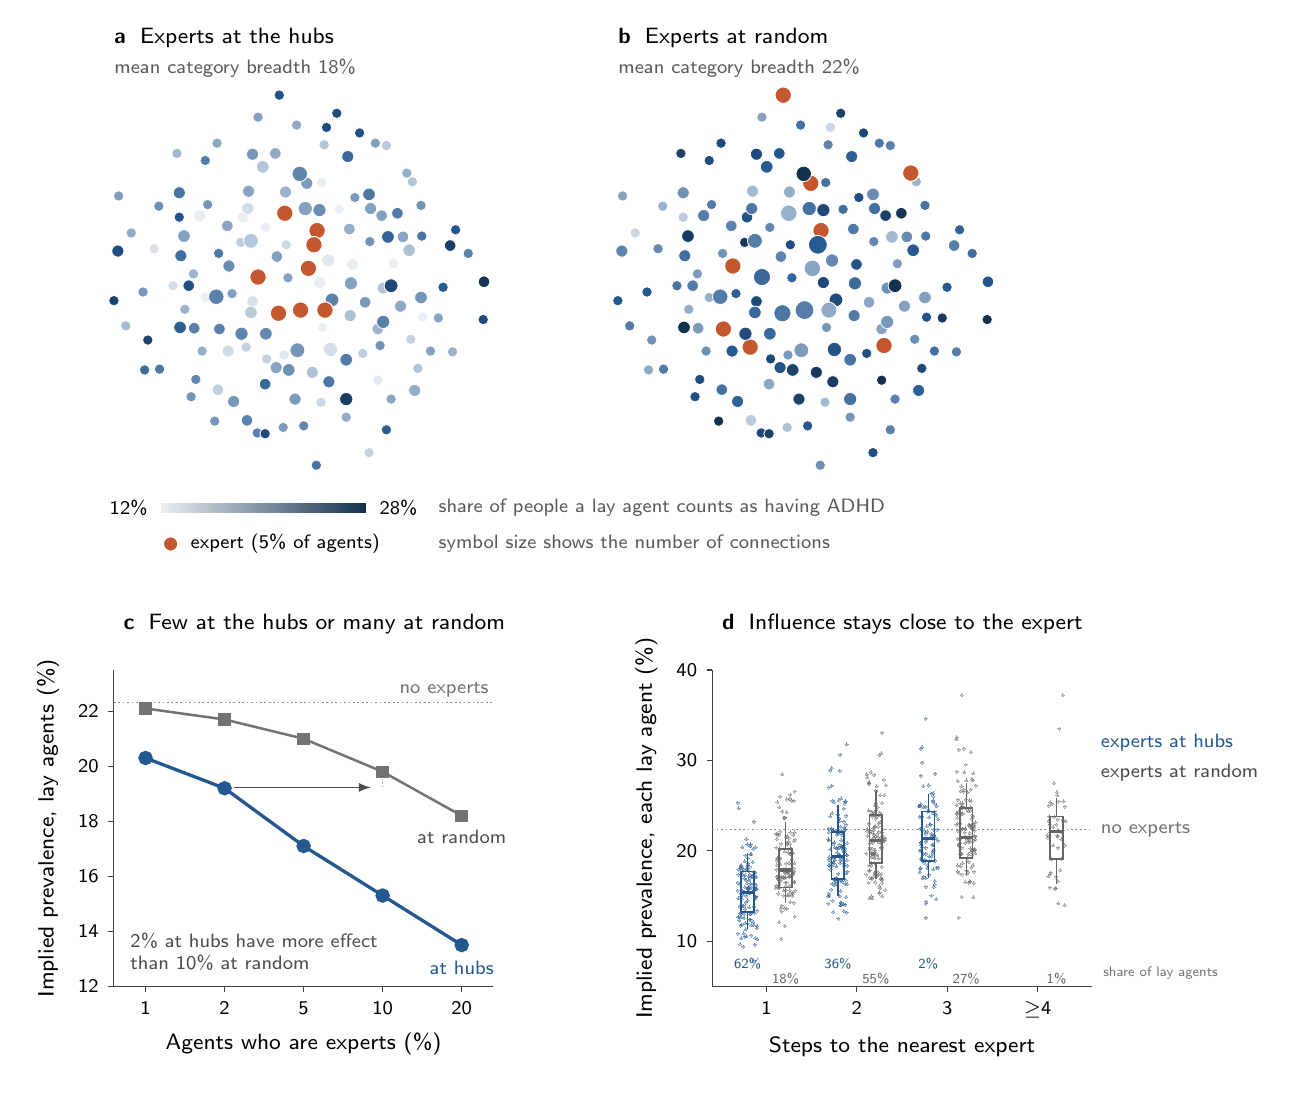
\begin{tikzpicture}[font=\sffamily\footnotesize]
\begin{scope}[xshift=0.0cm]
\begin{scope}[black!20,line width=0.25pt]\netedges\end{scope}
\filldraw[fill=cA!58!white,draw=white,line width=0.3pt] (3.32,4.09) circle (1.9pt);\filldraw[fill=cA!93!black,draw=white,line width=0.3pt] (3.12,4.22) circle (1.9pt);\filldraw[fill=cA!28!white,draw=white,line width=0.3pt] (1.94,1.35) circle (1.9pt);\filldraw[fill=cA!63!white,draw=white,line width=0.3pt] (0.37,2.20) circle (1.9pt);\filldraw[fill=cA!89!white,draw=white,line width=0.3pt] (0.39,1.21) circle (1.9pt);\filldraw[fill=cA!64!white,draw=white,line width=0.3pt] (0.98,0.87) circle (1.9pt);\filldraw[fill=cA!45!white,draw=white,line width=0.3pt] (1.01,2.43) circle (1.9pt);\filldraw[fill=cA!62!white,draw=white,line width=0.3pt] (1.28,0.56) circle (1.9pt);\filldraw[fill=cA!84!white,draw=white,line width=0.3pt] (3.91,2.91) circle (1.9pt);\filldraw[fill=cA!81!white,draw=white,line width=0.3pt] (0.58,1.22) circle (1.9pt);\filldraw[fill=cA!64!white,draw=white,line width=0.3pt] (3.38,1.52) circle (1.9pt);\filldraw[fill=cA!80!white,draw=white,line width=0.3pt] (1.33,2.69) circle (1.9pt);\filldraw[fill=cA!76!white,draw=white,line width=0.3pt] (1.82,0.41) circle (1.9pt);\filldraw[fill=cA!49!white,draw=white,line width=0.3pt] (1.12,1.45) circle (1.9pt);\filldraw[fill=cA!72!white,draw=white,line width=0.3pt] (2.41,0.50) circle (1.9pt);\filldraw[fill=cA!30!white,draw=white,line width=0.3pt] (1.61,2.83) circle (1.9pt);\filldraw[fill=cA!89!black,draw=white,line width=0.3pt] (2.70,4.29) circle (1.9pt);\filldraw[fill=cA!62!white,draw=white,line width=0.3pt] (1.19,3.31) circle (1.9pt);\filldraw[fill=cA!55!white,draw=white,line width=0.3pt] (2.21,2.38) circle (1.9pt);\filldraw[fill=cA!75!black,draw=white,line width=0.3pt] (0.00,2.09) circle (1.9pt);\filldraw[fill=cA!57!white,draw=white,line width=0.3pt] (1.50,2.18) circle (1.9pt);\filldraw[fill=cA!43!white,draw=white,line width=0.3pt] (0.80,3.96) circle (1.9pt);\filldraw[fill=cA!79!black,draw=white,line width=0.3pt] (0.43,1.59) circle (1.9pt);\filldraw[fill=cA!92!black,draw=white,line width=0.3pt] (2.10,4.70) circle (1.9pt);\filldraw[fill=cA!87!black,draw=white,line width=0.3pt] (2.83,4.47) circle (1.9pt);\filldraw[fill=cA!99!white,draw=white,line width=0.3pt] (4.18,2.26) circle (1.9pt);\filldraw[fill=cA!29!white,draw=white,line width=0.3pt] (3.16,1.42) circle (1.9pt);\filldraw[fill=cA!77!white,draw=white,line width=0.3pt] (1.16,3.87) circle (1.9pt);\filldraw[fill=cA!33!white,draw=white,line width=0.3pt] (3.46,4.06) circle (1.9pt);\filldraw[fill=cA!84!black,draw=white,line width=0.3pt] (1.92,0.40) circle (1.9pt);\filldraw[fill=cA!28!white,draw=white,line width=0.3pt] (1.68,1.50) circle (1.9pt);\filldraw[fill=cA!72!white,draw=white,line width=0.3pt] (1.04,1.09) circle (1.9pt);\filldraw[fill=cA!10!white,draw=white,line width=0.3pt] (3.92,1.88) circle (1.9pt);\filldraw[fill=cA!10!white,draw=white,line width=0.3pt] (3.55,2.56) circle (1.9pt);\filldraw[fill=cA!98!black,draw=white,line width=0.3pt] (4.34,2.99) circle (1.9pt);\filldraw[fill=cA!34!white,draw=white,line width=0.3pt] (2.67,4.07) circle (1.9pt);\filldraw[fill=cA!13!white,draw=white,line width=0.3pt] (3.35,1.08) circle (1.9pt);\filldraw[fill=cA!53!white,draw=white,line width=0.3pt] (3.52,0.84) circle (1.9pt);\filldraw[fill=cA!67!white,draw=white,line width=0.3pt] (0.57,3.29) circle (1.9pt);\filldraw[fill=cA!86!black,draw=white,line width=0.3pt] (4.69,1.85) circle (1.9pt);\filldraw[fill=cA!96!black,draw=white,line width=0.3pt] (0.83,3.15) circle (1.9pt);\filldraw[fill=cA!60!white,draw=white,line width=0.3pt] (2.15,0.48) circle (1.9pt);\filldraw[fill=cA!54!white,draw=white,line width=0.3pt] (4.12,1.87) circle (1.9pt);\filldraw[fill=cA!55!white,draw=white,line width=0.3pt] (4.02,1.45) circle (1.9pt);\filldraw[fill=cA!10!white,draw=white,line width=0.3pt] (1.16,2.13) circle (1.9pt);\filldraw[fill=cA!50!white,draw=white,line width=0.3pt] (2.95,0.61) circle (1.9pt);\filldraw[fill=cA!75!white,draw=white,line width=0.3pt] (4.50,2.69) circle (1.9pt);\filldraw[fill=cA!23!white,draw=white,line width=0.3pt] (2.19,2.80) circle (1.9pt);\filldraw[fill=cA!36!white,draw=white,line width=0.3pt] (3.86,1.23) circle (1.9pt);\filldraw[fill=cA!40!white,draw=white,line width=0.3pt] (0.15,1.77) circle (1.9pt);\filldraw[fill=cA!96!white,draw=white,line width=0.3pt] (3.46,0.45) circle (1.9pt);\filldraw[fill=cA!15!white,draw=white,line width=0.3pt] (2.16,1.40) circle (1.9pt);\filldraw[fill=cA!24!white,draw=white,line width=0.3pt] (2.63,0.80) circle (1.9pt);\filldraw[fill=cA!34!white,draw=white,line width=0.3pt] (3.79,3.60) circle (1.9pt);\filldraw[fill=cA!64!white,draw=white,line width=0.3pt] (3.25,2.84) circle (1.9pt);\filldraw[fill=cA!20!white,draw=white,line width=0.3pt] (0.75,2.28) circle (1.9pt);\filldraw[fill=cA!26!white,draw=white,line width=0.3pt] (3.24,0.16) circle (1.9pt);\filldraw[fill=cA!84!white,draw=white,line width=0.3pt] (2.57,0.00) circle (1.9pt);\filldraw[fill=cA!27!white,draw=white,line width=0.3pt] (3.77,1.60) circle (1.9pt);\filldraw[fill=cA!49!white,draw=white,line width=0.3pt] (3.72,3.71) circle (1.9pt);\filldraw[fill=cA!51!white,draw=white,line width=0.3pt] (0.22,2.95) circle (1.9pt);\filldraw[fill=cA!56!white,draw=white,line width=0.3pt] (1.83,4.42) circle (1.9pt);\filldraw[fill=cA!45!white,draw=white,line width=0.3pt] (4.30,1.44) circle (1.9pt);\filldraw[fill=cA!60!white,draw=white,line width=0.3pt] (3.06,3.40) circle (1.9pt);\filldraw[fill=cA!10!white,draw=white,line width=0.3pt] (2.65,1.75) circle (1.9pt);\filldraw[fill=cA!10!white,draw=white,line width=0.3pt] (2.64,3.59) circle (1.9pt);\filldraw[fill=cA!45!white,draw=white,line width=0.3pt] (0.90,1.98) circle (1.9pt);\filldraw[fill=cA!59!white,draw=white,line width=0.3pt] (0.06,3.42) circle (1.9pt);\filldraw[fill=cA!11!white,draw=white,line width=0.3pt] (1.93,3.02) circle (1.9pt);\filldraw[fill=cA!66!white,draw=white,line width=0.3pt] (3.90,3.30) circle (1.9pt);\filldraw[fill=cA!18!white,draw=white,line width=0.3pt] (0.51,2.75) circle (1.9pt);\filldraw[fill=cA!10!white,draw=white,line width=0.3pt] (2.86,3.25) circle (1.9pt);\filldraw[fill=cA!51!white,draw=white,line width=0.3pt] (2.32,4.32) circle (1.9pt);\filldraw[fill=cA!52!white,draw=white,line width=0.3pt] (1.31,4.09) circle (1.9pt);\filldraw[fill=cA!92!white,draw=white,line width=0.3pt] (1.92,1.03) circle (2.1pt);\filldraw[fill=cA!48!white,draw=white,line width=0.3pt] (2.99,3.00) circle (2.1pt);\filldraw[fill=cA!76!white,draw=white,line width=0.3pt] (1.34,1.73) circle (2.1pt);\filldraw[fill=cA!57!white,draw=white,line width=0.3pt] (2.07,2.65) circle (2.1pt);\filldraw[fill=cA!61!white,draw=white,line width=0.3pt] (3.19,2.07) circle (2.1pt);\filldraw[fill=cA!56!white,draw=white,line width=0.3pt] (3.40,3.17) circle (2.1pt);\filldraw[fill=cA!11!white,draw=white,line width=0.3pt] (3.03,2.55) circle (2.1pt);\filldraw[fill=cA!79!white,draw=white,line width=0.3pt] (3.60,3.20) circle (2.1pt);\filldraw[fill=cA!72!black,draw=white,line width=0.3pt] (4.27,2.79) circle (2.1pt);\filldraw[fill=cA!76!white,draw=white,line width=0.3pt] (1.02,1.74) circle (2.1pt);\filldraw[fill=cA!60!black,draw=white,line width=0.3pt] (4.70,2.33) circle (2.1pt);\filldraw[fill=cA!50!white,draw=white,line width=0.3pt] (2.05,3.96) circle (2.1pt);\filldraw[fill=cA!54!white,draw=white,line width=0.3pt] (1.44,3.04) circle (2.1pt);\filldraw[fill=cA!54!white,draw=white,line width=0.3pt] (3.67,2.90) circle (2.1pt);\filldraw[fill=cA!44!white,draw=white,line width=0.3pt] (3.35,1.73) circle (2.1pt);\filldraw[fill=cA!18!white,draw=white,line width=0.3pt] (1.76,2.08) circle (2.1pt);\filldraw[fill=cA!10!white,draw=white,line width=0.3pt] (1.64,3.15) circle (2.1pt);\filldraw[fill=cA!75!white,draw=white,line width=0.3pt] (1.69,0.57) circle (2.1pt);\filldraw[fill=cA!91!black,draw=white,line width=0.3pt] (0.95,2.28) circle (2.1pt);\filldraw[fill=cA!29!white,draw=white,line width=0.3pt] (1.32,0.96) circle (2.1pt);\filldraw[fill=cA!57!white,draw=white,line width=0.3pt] (3.26,3.26) circle (2.2pt);\filldraw[fill=cA!35!white,draw=white,line width=0.3pt] (3.42,2.25) circle (2.2pt);\filldraw[fill=cA!54!white,draw=white,line width=0.3pt] (1.71,3.48) circle (2.2pt);\filldraw[fill=cA!81!white,draw=white,line width=0.3pt] (2.73,1.06) circle (2.2pt);\filldraw[fill=cA!46!white,draw=white,line width=0.3pt] (2.18,3.47) circle (2.2pt);\filldraw[fill=cA!21!white,draw=white,line width=0.3pt] (1.70,3.26) circle (2.2pt);\filldraw[fill=cA!21!white,draw=white,line width=0.3pt] (1.45,1.45) circle (2.2pt);\filldraw[fill=cA!60!white,draw=white,line width=0.3pt] (2.30,0.84) circle (2.2pt);\filldraw[fill=cA!60!white,draw=white,line width=0.3pt] (2.45,3.58) circle (2.2pt);\filldraw[fill=cA!49!white,draw=white,line width=0.3pt] (3.82,0.95) circle (2.2pt);\filldraw[fill=cA!37!white,draw=white,line width=0.3pt] (2.52,1.18) circle (2.2pt);\filldraw[fill=cA!87!white,draw=white,line width=0.3pt] (0.85,2.66) circle (2.2pt);\filldraw[fill=cA!89!white,draw=white,line width=0.3pt] (2.97,3.92) circle (2.2pt);\filldraw[fill=cA!38!white,draw=white,line width=0.3pt] (3.00,1.90) circle (2.2pt);\filldraw[fill=cA!88!black,draw=white,line width=0.3pt] (0.05,2.72) circle (2.2pt);\filldraw[fill=cA!84!white,draw=white,line width=0.3pt] (0.83,3.46) circle (2.2pt);\filldraw[fill=cA!10!white,draw=white,line width=0.3pt] (1.09,3.17) circle (2.2pt);\filldraw[fill=cA!10!white,draw=white,line width=0.3pt] (2.61,2.32) circle (2.2pt);\filldraw[fill=cA!63!white,draw=white,line width=0.3pt] (1.76,3.95) circle (2.2pt);\filldraw[fill=cA!55!white,draw=white,line width=0.3pt] (2.06,1.24) circle (2.2pt);\filldraw[fill=cA!69!white,draw=white,line width=0.3pt] (1.46,2.53) circle (2.2pt);\filldraw[fill=cA!52!white,draw=white,line width=0.3pt] (3.64,2.02) circle (2.2pt);\filldraw[fill=cA!62!white,draw=white,line width=0.3pt] (1.52,0.81) circle (2.2pt);\filldraw[fill=cA!31!white,draw=white,line width=0.3pt] (1.74,1.94) circle (2.3pt);\filldraw[fill=cA!71!white,draw=white,line width=0.3pt] (1.93,1.67) circle (2.3pt);\filldraw[fill=cA!38!white,draw=white,line width=0.3pt] (3.75,2.73) circle (2.3pt);\filldraw[fill=cA!67!white,draw=white,line width=0.3pt] (2.22,1.21) circle (2.3pt);\filldraw[fill=cA!93!white,draw=white,line width=0.3pt] (3.48,2.90) circle (2.3pt);\filldraw[fill=cA!96!white,draw=white,line width=0.3pt] (0.84,1.75) circle (2.3pt);\filldraw[fill=cA!79!white,draw=white,line width=0.3pt] (2.95,1.34) circle (2.3pt);\filldraw[fill=cA!64!white,draw=white,line width=0.3pt] (3.90,2.13) circle (2.3pt);\filldraw[fill=cA!35!white,draw=white,line width=0.3pt] (1.89,3.79) circle (2.3pt);\filldraw[fill=cA!81!white,draw=white,line width=0.3pt] (3.24,3.44) circle (2.3pt);\filldraw[fill=cA!56!white,draw=white,line width=0.3pt] (0.89,2.91) circle (2.3pt);\filldraw[fill=cA!69!white,draw=white,line width=0.3pt] (2.61,3.24) circle (2.4pt);\filldraw[fill=cA!76!white,draw=white,line width=0.3pt] (3.42,1.82) circle (2.4pt);\filldraw[fill=cA!14!white,draw=white,line width=0.3pt] (2.72,2.60) circle (2.4pt);\filldraw[fill=cA!73!white,draw=white,line width=0.3pt] (1.62,1.67) circle (2.4pt);\filldraw[fill=cA!72!black,draw=white,line width=0.3pt] (2.95,0.84) circle (2.4pt);\filldraw[fill=cA!56!white,draw=white,line width=0.3pt] (3.01,2.31) circle (2.4pt);\filldraw[fill=cA!82!black,draw=white,line width=0.3pt] (3.52,2.28) circle (2.5pt);\filldraw[fill=cA!74!white,draw=white,line width=0.3pt] (2.77,2.10) circle (2.5pt);\filldraw[fill=cA!56!white,draw=white,line width=0.3pt] (2.43,3.26) circle (2.6pt);\filldraw[fill=cA!19!white,draw=white,line width=0.3pt] (2.75,1.47) circle (2.6pt);\filldraw[fill=cA!63!white,draw=white,line width=0.3pt] (2.33,1.46) circle (2.7pt);\filldraw[fill=cA!33!white,draw=white,line width=0.3pt] (1.74,2.85) circle (2.7pt);\filldraw[fill=cB,draw=white,line width=0.4pt] (2.58,2.98) circle (3.0pt);\filldraw[fill=cA!73!white,draw=white,line width=0.3pt] (2.36,3.70) circle (2.8pt);\filldraw[fill=cA!75!white,draw=white,line width=0.3pt] (1.30,2.14) circle (2.8pt);\filldraw[fill=cB,draw=white,line width=0.4pt] (2.68,1.97) circle (3.0pt);\filldraw[fill=cB,draw=white,line width=0.4pt] (2.17,3.20) circle (3.0pt);\filldraw[fill=cB,draw=white,line width=0.4pt] (2.47,2.50) circle (3.0pt);\filldraw[fill=cB,draw=white,line width=0.4pt] (1.83,2.39) circle (3.0pt);\filldraw[fill=cB,draw=white,line width=0.4pt] (2.09,1.93) circle (3.0pt);\filldraw[fill=cB,draw=white,line width=0.4pt] (2.54,2.80) circle (3.0pt);\filldraw[fill=cB,draw=white,line width=0.4pt] (2.37,1.97) circle (3.0pt);
\node[anchor=south west,inner sep=0pt] at (0,5.3) {\textbf{a}\hspace{0.6em}Experts at the hubs};
\node[font=\sffamily\scriptsize,anchor=south west,inner sep=0pt,text=black!65] at (0,4.92) {mean category breadth 18\%};
\end{scope}
\begin{scope}[xshift=6.4cm]
\begin{scope}[black!20,line width=0.25pt]\netedges\end{scope}
\filldraw[fill=cA!81!white,draw=white,line width=0.3pt] (3.32,4.09) circle (1.9pt);\filldraw[fill=cA!81!black,draw=white,line width=0.3pt] (3.12,4.22) circle (1.9pt);\filldraw[fill=cA!82!black,draw=white,line width=0.3pt] (1.94,1.35) circle (1.9pt);\filldraw[fill=cA!99!black,draw=white,line width=0.3pt] (0.37,2.20) circle (1.9pt);\filldraw[fill=cA!50!white,draw=white,line width=0.3pt] (0.39,1.21) circle (1.9pt);\filldraw[fill=cA!89!black,draw=white,line width=0.3pt] (0.98,0.87) circle (1.9pt);\filldraw[fill=cA!60!white,draw=white,line width=0.3pt] (1.01,2.43) circle (1.9pt);\filldraw[fill=cA!54!black,draw=white,line width=0.3pt] (1.28,0.56) circle (1.9pt);\filldraw[fill=cA!82!white,draw=white,line width=0.3pt] (3.91,2.91) circle (1.9pt);\filldraw[fill=cA!80!white,draw=white,line width=0.3pt] (0.58,1.22) circle (1.9pt);\filldraw[fill=cB,draw=white,line width=0.4pt] (3.38,1.52) circle (3.0pt);\filldraw[fill=cA!66!white,draw=white,line width=0.3pt] (1.33,2.69) circle (1.9pt);\filldraw[fill=cA!82!black,draw=white,line width=0.3pt] (1.82,0.41) circle (1.9pt);\filldraw[fill=cA!67!white,draw=white,line width=0.3pt] (1.12,1.45) circle (1.9pt);\filldraw[fill=cA!99!white,draw=white,line width=0.3pt] (2.41,0.50) circle (1.9pt);\filldraw[fill=cA!61!black,draw=white,line width=0.3pt] (1.61,2.83) circle (1.9pt);\filldraw[fill=cA!24!white,draw=white,line width=0.3pt] (2.70,4.29) circle (1.9pt);\filldraw[fill=cA!79!white,draw=white,line width=0.3pt] (1.19,3.31) circle (1.9pt);\filldraw[fill=cA!93!white,draw=white,line width=0.3pt] (2.21,2.38) circle (1.9pt);\filldraw[fill=cA!99!black,draw=white,line width=0.3pt] (0.00,2.09) circle (1.9pt);\filldraw[fill=cA!96!white,draw=white,line width=0.3pt] (1.50,2.18) circle (1.9pt);\filldraw[fill=cA!76!black,draw=white,line width=0.3pt] (0.80,3.96) circle (1.9pt);\filldraw[fill=cA!65!white,draw=white,line width=0.3pt] (0.43,1.59) circle (1.9pt);\filldraw[fill=cB,draw=white,line width=0.4pt] (2.10,4.70) circle (3.0pt);\filldraw[fill=cA!75!black,draw=white,line width=0.3pt] (2.83,4.47) circle (1.9pt);\filldraw[fill=cA!99!white,draw=white,line width=0.3pt] (4.18,2.26) circle (1.9pt);\filldraw[fill=cA!90!black,draw=white,line width=0.3pt] (3.16,1.42) circle (1.9pt);\filldraw[fill=cA!88!black,draw=white,line width=0.3pt] (1.16,3.87) circle (1.9pt);\filldraw[fill=cA!76!white,draw=white,line width=0.3pt] (3.46,4.06) circle (1.9pt);\filldraw[fill=cA!73!black,draw=white,line width=0.3pt] (1.92,0.40) circle (1.9pt);\filldraw[fill=cB,draw=white,line width=0.4pt] (1.68,1.50) circle (3.0pt);\filldraw[fill=cA!86!black,draw=white,line width=0.3pt] (1.04,1.09) circle (1.9pt);\filldraw[fill=cA!94!black,draw=white,line width=0.3pt] (3.92,1.88) circle (1.9pt);\filldraw[fill=cA!58!white,draw=white,line width=0.3pt] (3.55,2.56) circle (1.9pt);\filldraw[fill=cA!93!white,draw=white,line width=0.3pt] (4.34,2.99) circle (1.9pt);\filldraw[fill=cA!73!white,draw=white,line width=0.3pt] (2.67,4.07) circle (1.9pt);\filldraw[fill=cA!54!black,draw=white,line width=0.3pt] (3.35,1.08) circle (1.9pt);\filldraw[fill=cA!75!white,draw=white,line width=0.3pt] (3.52,0.84) circle (1.9pt);\filldraw[fill=cA!46!white,draw=white,line width=0.3pt] (0.57,3.29) circle (1.9pt);\filldraw[fill=cA!54!black,draw=white,line width=0.3pt] (4.69,1.85) circle (1.9pt);\filldraw[fill=cA!31!white,draw=white,line width=0.3pt] (0.83,3.15) circle (1.9pt);\filldraw[fill=cA!38!white,draw=white,line width=0.3pt] (2.15,0.48) circle (1.9pt);\filldraw[fill=cA!64!black,draw=white,line width=0.3pt] (4.12,1.87) circle (1.9pt);\filldraw[fill=cA!86!white,draw=white,line width=0.3pt] (4.02,1.45) circle (1.9pt);\filldraw[fill=cA!48!white,draw=white,line width=0.3pt] (1.16,2.13) circle (1.9pt);\filldraw[fill=cA!63!white,draw=white,line width=0.3pt] (2.95,0.61) circle (1.9pt);\filldraw[fill=cA!88!white,draw=white,line width=0.3pt] (4.50,2.69) circle (1.9pt);\filldraw[fill=cA!87!black,draw=white,line width=0.3pt] (2.19,2.80) circle (1.9pt);\filldraw[fill=cA!82!black,draw=white,line width=0.3pt] (3.86,1.23) circle (1.9pt);\filldraw[fill=cA!79!white,draw=white,line width=0.3pt] (0.15,1.77) circle (1.9pt);\filldraw[fill=cA!76!white,draw=white,line width=0.3pt] (3.46,0.45) circle (1.9pt);\filldraw[fill=cA!61!white,draw=white,line width=0.3pt] (2.16,1.40) circle (1.9pt);\filldraw[fill=cA!41!white,draw=white,line width=0.3pt] (2.63,0.80) circle (1.9pt);\filldraw[fill=cA!45!white,draw=white,line width=0.3pt] (3.79,3.60) circle (1.9pt);\filldraw[fill=cA!71!white,draw=white,line width=0.3pt] (3.25,2.84) circle (1.9pt);\filldraw[fill=cA!84!white,draw=white,line width=0.3pt] (0.75,2.28) circle (1.9pt);\filldraw[fill=cA!86!black,draw=white,line width=0.3pt] (3.24,0.16) circle (1.9pt);\filldraw[fill=cA!65!white,draw=white,line width=0.3pt] (2.57,0.00) circle (1.9pt);\filldraw[fill=cA!67!white,draw=white,line width=0.3pt] (3.77,1.60) circle (1.9pt);\filldraw[fill=cB,draw=white,line width=0.4pt] (3.72,3.71) circle (3.0pt);\filldraw[fill=cA!24!white,draw=white,line width=0.3pt] (0.22,2.95) circle (1.9pt);\filldraw[fill=cA!55!white,draw=white,line width=0.3pt] (1.83,4.42) circle (1.9pt);\filldraw[fill=cA!78!white,draw=white,line width=0.3pt] (4.30,1.44) circle (1.9pt);\filldraw[fill=cA!89!black,draw=white,line width=0.3pt] (3.06,3.40) circle (1.9pt);\filldraw[fill=cA!62!white,draw=white,line width=0.3pt] (2.65,1.75) circle (1.9pt);\filldraw[fill=cA!84!white,draw=white,line width=0.3pt] (2.64,3.59) circle (1.9pt);\filldraw[fill=cA!49!white,draw=white,line width=0.3pt] (0.90,1.98) circle (1.9pt);\filldraw[fill=cA!55!white,draw=white,line width=0.3pt] (0.06,3.42) circle (1.9pt);\filldraw[fill=cA!71!white,draw=white,line width=0.3pt] (1.93,3.02) circle (1.9pt);\filldraw[fill=cA!83!white,draw=white,line width=0.3pt] (3.90,3.30) circle (1.9pt);\filldraw[fill=cA!70!white,draw=white,line width=0.3pt] (0.51,2.75) circle (1.9pt);\filldraw[fill=cA!86!white,draw=white,line width=0.3pt] (2.86,3.25) circle (1.9pt);\filldraw[fill=cA!85!white,draw=white,line width=0.3pt] (2.32,4.32) circle (1.9pt);\filldraw[fill=cA!84!black,draw=white,line width=0.3pt] (1.31,4.09) circle (1.9pt);\filldraw[fill=cA!52!white,draw=white,line width=0.3pt] (1.92,1.03) circle (2.1pt);\filldraw[fill=cA!80!white,draw=white,line width=0.3pt] (2.99,3.00) circle (2.1pt);\filldraw[fill=cB,draw=white,line width=0.4pt] (1.34,1.73) circle (3.0pt);\filldraw[fill=cA!73!white,draw=white,line width=0.3pt] (2.07,2.65) circle (2.1pt);\filldraw[fill=cA!53!white,draw=white,line width=0.3pt] (3.19,2.07) circle (2.1pt);\filldraw[fill=cA!73!black,draw=white,line width=0.3pt] (3.40,3.17) circle (2.1pt);\filldraw[fill=cA!94!black,draw=white,line width=0.3pt] (3.03,2.55) circle (2.1pt);\filldraw[fill=cA!61!black,draw=white,line width=0.3pt] (3.60,3.20) circle (2.1pt);\filldraw[fill=cA!77!white,draw=white,line width=0.3pt] (4.27,2.79) circle (2.1pt);\filldraw[fill=cA!61!white,draw=white,line width=0.3pt] (1.02,1.74) circle (2.1pt);\filldraw[fill=cA!97!black,draw=white,line width=0.3pt] (4.70,2.33) circle (2.1pt);\filldraw[fill=cA!98!black,draw=white,line width=0.3pt] (2.05,3.96) circle (2.1pt);\filldraw[fill=cA!74!white,draw=white,line width=0.3pt] (1.44,3.04) circle (2.1pt);\filldraw[fill=cA!70!white,draw=white,line width=0.3pt] (3.67,2.90) circle (2.1pt);\filldraw[fill=cA!55!white,draw=white,line width=0.3pt] (3.35,1.73) circle (2.1pt);\filldraw[fill=cA!84!black,draw=white,line width=0.3pt] (1.76,2.08) circle (2.1pt);\filldraw[fill=cA!94!black,draw=white,line width=0.3pt] (1.64,3.15) circle (2.1pt);\filldraw[fill=cA!31!white,draw=white,line width=0.3pt] (1.69,0.57) circle (2.1pt);\filldraw[fill=cA!79!white,draw=white,line width=0.3pt] (0.95,2.28) circle (2.1pt);\filldraw[fill=cA!85!white,draw=white,line width=0.3pt] (1.32,0.96) circle (2.1pt);\filldraw[fill=cA!87!white,draw=white,line width=0.3pt] (3.26,3.26) circle (2.2pt);\filldraw[fill=cA!67!white,draw=white,line width=0.3pt] (3.42,2.25) circle (2.2pt);\filldraw[fill=cA!42!white,draw=white,line width=0.3pt] (1.71,3.48) circle (2.2pt);\filldraw[fill=cA!68!black,draw=white,line width=0.3pt] (2.73,1.06) circle (2.2pt);\filldraw[fill=cA!48!white,draw=white,line width=0.3pt] (2.18,3.47) circle (2.2pt);\filldraw[fill=cA!82!white,draw=white,line width=0.3pt] (1.70,3.26) circle (2.2pt);\filldraw[fill=cA!98!white,draw=white,line width=0.3pt] (1.45,1.45) circle (2.2pt);\filldraw[fill=cA!74!black,draw=white,line width=0.3pt] (2.30,0.84) circle (2.2pt);\filldraw[fill=cB,draw=white,line width=0.4pt] (2.45,3.58) circle (3.0pt);\filldraw[fill=cA!95!white,draw=white,line width=0.3pt] (3.82,0.95) circle (2.2pt);\filldraw[fill=cA!62!black,draw=white,line width=0.3pt] (2.52,1.18) circle (2.2pt);\filldraw[fill=cA!87!white,draw=white,line width=0.3pt] (0.85,2.66) circle (2.2pt);\filldraw[fill=cA!96!white,draw=white,line width=0.3pt] (2.97,3.92) circle (2.2pt);\filldraw[fill=cA!80!white,draw=white,line width=0.3pt] (3.00,1.90) circle (2.2pt);\filldraw[fill=cA!73!white,draw=white,line width=0.3pt] (0.05,2.72) circle (2.2pt);\filldraw[fill=cA!66!white,draw=white,line width=0.3pt] (0.83,3.46) circle (2.2pt);\filldraw[fill=cA!78!white,draw=white,line width=0.3pt] (1.09,3.17) circle (2.2pt);\filldraw[fill=cA!81!black,draw=white,line width=0.3pt] (2.61,2.32) circle (2.2pt);\filldraw[fill=cA!85!black,draw=white,line width=0.3pt] (1.76,3.95) circle (2.2pt);\filldraw[fill=cA!94!black,draw=white,line width=0.3pt] (2.06,1.24) circle (2.2pt);\filldraw[fill=cB,draw=white,line width=0.4pt] (1.46,2.53) circle (3.0pt);\filldraw[fill=cA!57!white,draw=white,line width=0.3pt] (3.64,2.02) circle (2.2pt);\filldraw[fill=cA!94!white,draw=white,line width=0.3pt] (1.52,0.81) circle (2.2pt);\filldraw[fill=cA!91!white,draw=white,line width=0.3pt] (1.74,1.94) circle (2.3pt);\filldraw[fill=cA!91!white,draw=white,line width=0.3pt] (1.93,1.67) circle (2.3pt);\filldraw[fill=cA!99!white,draw=white,line width=0.3pt] (3.75,2.73) circle (2.3pt);\filldraw[fill=cA!74!black,draw=white,line width=0.3pt] (2.22,1.21) circle (2.3pt);\filldraw[fill=cA!42!white,draw=white,line width=0.3pt] (3.48,2.90) circle (2.3pt);\filldraw[fill=cA!54!black,draw=white,line width=0.3pt] (0.84,1.75) circle (2.3pt);\filldraw[fill=cA!83!white,draw=white,line width=0.3pt] (2.95,1.34) circle (2.3pt);\filldraw[fill=cA!57!white,draw=white,line width=0.3pt] (3.90,2.13) circle (2.3pt);\filldraw[fill=cA!99!white,draw=white,line width=0.3pt] (1.89,3.79) circle (2.3pt);\filldraw[fill=cA!69!white,draw=white,line width=0.3pt] (3.24,3.44) circle (2.3pt);\filldraw[fill=cA!67!black,draw=white,line width=0.3pt] (0.89,2.91) circle (2.3pt);\filldraw[fill=cA!81!black,draw=white,line width=0.3pt] (2.61,3.24) circle (2.4pt);\filldraw[fill=cA!62!white,draw=white,line width=0.3pt] (3.42,1.82) circle (2.4pt);\filldraw[fill=cA!71!white,draw=white,line width=0.3pt] (2.72,2.60) circle (2.4pt);\filldraw[fill=cA!88!black,draw=white,line width=0.3pt] (1.62,1.67) circle (2.4pt);\filldraw[fill=cA!85!white,draw=white,line width=0.3pt] (2.95,0.84) circle (2.4pt);\filldraw[fill=cA!89!white,draw=white,line width=0.3pt] (3.01,2.31) circle (2.4pt);\filldraw[fill=cA!54!black,draw=white,line width=0.3pt] (3.52,2.28) circle (2.5pt);\filldraw[fill=cA!86!black,draw=white,line width=0.3pt] (2.77,2.10) circle (2.5pt);\filldraw[fill=cA!85!white,draw=white,line width=0.3pt] (2.43,3.26) circle (2.6pt);\filldraw[fill=cA!94!black,draw=white,line width=0.3pt] (2.75,1.47) circle (2.6pt);\filldraw[fill=cA!60!white,draw=white,line width=0.3pt] (2.33,1.46) circle (2.7pt);\filldraw[fill=cA!78!white,draw=white,line width=0.3pt] (1.74,2.85) circle (2.7pt);\filldraw[fill=cB,draw=white,line width=0.4pt] (2.58,2.98) circle (3.0pt);\filldraw[fill=cA!54!black,draw=white,line width=0.3pt] (2.36,3.70) circle (2.8pt);\filldraw[fill=cA!79!white,draw=white,line width=0.3pt] (1.30,2.14) circle (2.8pt);\filldraw[fill=cA!50!white,draw=white,line width=0.3pt] (2.68,1.97) circle (2.9pt);\filldraw[fill=cA!47!white,draw=white,line width=0.3pt] (2.17,3.20) circle (3.0pt);\filldraw[fill=cA!54!white,draw=white,line width=0.3pt] (2.47,2.50) circle (3.0pt);\filldraw[fill=cA!90!white,draw=white,line width=0.3pt] (1.83,2.39) circle (3.1pt);\filldraw[fill=cA!82!white,draw=white,line width=0.3pt] (2.09,1.93) circle (3.1pt);\filldraw[fill=cA!98!white,draw=white,line width=0.3pt] (2.54,2.80) circle (3.4pt);\filldraw[fill=cA!78!white,draw=white,line width=0.3pt] (2.37,1.97) circle (3.4pt);
\node[anchor=south west,inner sep=0pt] at (0,5.3) {\textbf{b}\hspace{0.6em}Experts at random};
\node[font=\sffamily\scriptsize,anchor=south west,inner sep=0pt,text=black!65] at (0,4.92) {mean category breadth 22\%};
\end{scope}
\shade[left color=cA!10!white,right color=cA!55!black] (0.6,-0.6) rectangle (3.2,-0.48);
\node[font=\sffamily\scriptsize,anchor=east] at (0.55,-0.54) {12\%};\node[font=\sffamily\scriptsize,anchor=west] at (3.25,-0.54) {28\%};
\node[font=\sffamily\scriptsize,anchor=west,text=black!65] at (4.0,-0.54) {share of people a lay agent counts as having ADHD};
\filldraw[fill=cB,draw=white] (0.72,-1.0) circle (2.6pt);\node[font=\sffamily\scriptsize,anchor=west] at (0.85,-1.0) {expert (5\% of agents)};
\node[font=\sffamily\scriptsize,anchor=west,text=black!65] at (4.0,-1.0) {symbol size shows the number of connections};
\begin{axis}[pub,at={(0cm,-2.6cm)},anchor=north west,width=6.4cm,height=5.6cm,title={\textbf{c}\hspace{0.6em}Few at the hubs or many at random},xlabel={Agents who are experts (\%)},ylabel={Implied prevalence, lay agents (\%)},xmin=0.6,xmax=5.4,ymin=12,ymax=23.5,xtick={1,...,5},xticklabels={1,2,5,10,20},ytick={12,14,...,22}]
\draw[black!45,densely dotted,line width=0.6pt] (axis cs:0.6,22.32) -- (axis cs:5.4,22.32);
\node[font=\sffamily\scriptsize,text=black!55,anchor=east,inner sep=1.5pt] at (axis cs:5.4,22.773686108571567) {no experts};
\addplot[black!55,mark=square*,mark size=1.8pt] coordinates {(1,22.1) (2,21.7) (3,21) (4,19.8) (5,18.2)};
\addplot[cA,mark=*,mark size=2pt,line width=1.2pt] coordinates {(1,20.3) (2,19.2) (3,17.1) (4,15.3) (5,13.5)};
\node[font=\sffamily\scriptsize,text=black!70,anchor=north,inner sep=1.5pt] at (axis cs:5.0,17.865362231637253) {at random};
\node[font=\sffamily\scriptsize,text=cA,anchor=north,inner sep=1.5pt] at (axis cs:5.0,13.102326248681454) {at hubs};
\draw[black!70,line width=0.5pt,-latex] (axis cs:2.12,19.23) -- (axis cs:3.85,19.23);
\draw[black!40,line width=0.4pt,densely dotted] (axis cs:4,19.23) -- (axis cs:4,19.77);
\node[font=\sffamily\scriptsize,text=black!70,anchor=south west,inner sep=1.5pt,align=left] at (axis cs:0.75,12.4) {2\% at hubs have more effect\\than 10\% at random};
\end{axis}
\begin{axis}[pub,at={(7.6cm,-2.6cm)},anchor=north west,width=6.4cm,height=5.6cm,title={\textbf{d}\hspace{0.6em}Influence stays close to the expert},xlabel={Steps to the nearest expert},ylabel={Implied prevalence, each lay agent (\%)},xmin=0.4,xmax=4.6,ymin=5,ymax=40,xtick={1,2,3,4},xticklabels={1,2,3,$\geq$4}]
\draw[black!45,densely dotted,line width=0.6pt] (axis cs:0.4,22.34) -- (axis cs:4.6,22.34);
\addplot[only marks,mark=*,mark size=0.55pt,cA,opacity=0.35,line width=0pt] coordinates {(0.818,20.48) (0.877,14.93) (0.851,20.18) (0.730,13.84) (0.746,17.96) (0.872,17.15) (0.681,10.84) (0.861,13.80) (0.855,16.25) (0.783,16.39) (0.747,13.90) (0.741,9.37) (0.736,17.70) (0.778,21.28) (0.791,14.51) (0.802,16.74) (0.899,13.37) (0.854,12.09) (0.817,12.96) (0.898,10.20) (0.727,11.82) (0.715,18.10) (0.815,17.36) (0.690,24.71) (0.688,17.35) (0.793,19.19) (0.783,17.93) (0.882,14.89) (0.818,16.06) (0.793,15.78) (0.789,20.72) (0.734,15.60) (0.683,25.30) (0.722,18.38) (0.832,19.63) (0.724,12.65) (0.761,15.97) (0.681,15.58) (0.863,16.36) (0.714,18.29) (0.739,17.30) (0.874,17.56) (0.792,11.94) (0.866,17.64) (0.821,16.39) (0.843,15.80) (0.700,12.31) (0.799,15.98) (0.792,18.40) (0.872,9.59) (0.759,10.48) (0.812,18.21) (0.693,12.68) (0.765,19.47) (0.751,12.99) (0.713,15.28) (0.860,23.22) (0.763,12.00) (0.895,11.67) (0.810,13.75) (0.813,12.38) (0.820,19.60) (0.829,10.62) (0.713,13.03) (0.777,10.55) (0.733,15.12) (0.769,11.32) (0.701,13.79) (0.893,11.43) (0.727,14.63) (0.828,13.04) (0.746,10.85) (0.872,14.63) (0.826,20.70) (0.709,13.09) (0.866,15.58) (0.888,16.21) (0.879,20.37) (0.805,17.15) (0.712,18.01) (0.722,14.99) (0.884,17.09) (0.802,15.33) (0.720,10.32) (0.874,15.72) (0.821,16.99) (0.805,17.73) (0.763,13.54) (0.770,14.23) (0.733,20.37) (0.688,17.90) (0.873,10.34) (0.783,18.08) (0.800,15.76) (0.751,12.55) (0.845,17.26) (0.686,12.66) (0.762,17.30) (0.687,14.73) (0.707,16.31) (0.893,15.72) (0.825,12.35) (0.774,15.03) (0.795,18.58) (0.872,13.10) (0.756,16.94) (0.810,15.30) (0.830,11.74) (0.758,18.83) (0.794,15.79) (0.848,18.73) (0.880,14.90) (0.713,11.72) (0.885,15.85) (0.681,16.46) (0.846,17.13) (0.858,11.77) (0.710,9.68) (0.772,16.76) (0.859,7.84)};
\draw[cA,line width=0.5pt] (axis cs:0.79,11.37) -- (axis cs:0.79,19.74);
\draw[cA,fill=white,line width=0.6pt] (axis cs:0.72,13.24) rectangle (axis cs:0.86,17.71);
\draw[cA,line width=1.1pt] (axis cs:0.72,15.37) -- (axis cs:0.86,15.37);
\node[font=\sffamily\tiny,text=cA] at (axis cs:0.79,7.5) {62\%};
\addplot[only marks,mark=*,mark size=0.55pt,cA,opacity=0.35,line width=0pt] coordinates {(1.683,14.15) (1.818,13.96) (1.854,24.66) (1.793,20.28) (1.840,16.60) (1.730,14.48) (1.724,22.32) (1.760,22.19) (1.719,18.77) (1.756,16.89) (1.889,19.51) (1.806,20.67) (1.755,20.37) (1.740,13.22) (1.889,18.95) (1.778,21.79) (1.896,17.70) (1.793,21.90) (1.795,17.43) (1.877,16.75) (1.843,20.43) (1.808,23.28) (1.774,18.29) (1.873,20.24) (1.771,17.01) (1.883,17.49) (1.695,19.29) (1.775,16.33) (1.794,12.50) (1.889,19.53) (1.735,18.58) (1.857,22.25) (1.829,21.16) (1.838,21.75) (1.819,13.96) (1.894,18.32) (1.753,16.68) (1.768,16.66) (1.725,24.13) (1.691,18.99) (1.727,16.34) (1.881,22.87) (1.865,25.21) (1.705,23.80) (1.813,14.95) (1.785,19.84) (1.811,22.23) (1.825,14.21) (1.747,25.35) (1.891,20.81) (1.782,22.01) (1.818,18.89) (1.820,15.54) (1.720,22.45) (1.694,15.04) (1.771,20.26) (1.848,18.95) (1.859,22.52) (1.841,20.11) (1.705,28.86) (1.881,23.85) (1.856,23.21) (1.873,25.47) (1.795,23.97) (1.881,14.87) (1.690,26.99) (1.687,22.41) (1.684,14.97) (1.736,22.26) (1.735,20.75) (1.721,29.15) (1.805,19.52) (1.689,22.04) (1.810,28.84) (1.717,15.70) (1.829,20.48) (1.685,21.28) (1.748,19.10) (1.886,13.16) (1.798,25.60) (1.859,20.61) (1.825,21.96) (1.814,18.62) (1.722,18.30) (1.806,23.56) (1.689,15.26) (1.856,19.83) (1.891,16.30) (1.868,19.97) (1.691,18.38) (1.755,18.95) (1.750,20.92) (1.705,20.15) (1.818,22.66) (1.855,14.06) (1.749,18.64) (1.870,14.04) (1.855,18.30) (1.708,17.91) (1.849,20.28) (1.874,25.47) (1.723,27.17) (1.806,20.32) (1.821,19.17) (1.814,30.61) (1.701,18.29) (1.825,25.79) (1.819,14.26) (1.861,18.55) (1.857,13.32) (1.752,16.18) (1.839,20.46) (1.871,16.35) (1.876,22.35) (1.716,18.64) (1.686,21.16) (1.823,16.68) (1.727,25.53) (1.804,19.57) (1.888,31.77)};
\draw[cA,line width=0.5pt] (axis cs:1.79,15.01) -- (axis cs:1.79,25.03);
\draw[cA,fill=white,line width=0.6pt] (axis cs:1.72,16.88) rectangle (axis cs:1.86,22.07);
\draw[cA,line width=1.1pt] (axis cs:1.72,19.39) -- (axis cs:1.86,19.39);
\node[font=\sffamily\tiny,text=cA] at (axis cs:1.79,7.5) {36\%};
\addplot[only marks,mark=*,mark size=0.55pt,cA,opacity=0.35,line width=0pt] coordinates {(2.763,14.15) (2.736,19.66) (2.780,24.34) (2.825,19.34) (2.702,18.09) (2.764,20.34) (2.709,20.86) (2.826,15.00) (2.863,16.64) (2.763,20.97) (2.762,34.62) (2.799,24.36) (2.727,16.96) (2.734,27.15) (2.753,19.03) (2.781,18.07) (2.698,20.02) (2.846,25.59) (2.807,18.85) (2.746,18.66) (2.697,17.61) (2.848,21.67) (2.709,25.13) (2.709,31.27) (2.709,19.07) (2.698,23.74) (2.879,23.90) (2.739,17.11) (2.747,22.24) (2.863,16.26) (2.816,22.89) (2.721,23.75) (2.776,22.73) (2.874,21.38) (2.763,21.86) (2.836,20.63) (2.701,24.96) (2.840,19.66) (2.851,15.99) (2.862,24.33) (2.828,21.63) (2.762,12.58) (2.694,24.94) (2.794,27.22) (2.847,17.96) (2.722,31.46) (2.739,24.82) (2.798,17.37) (2.845,26.36) (2.877,14.63) (2.708,28.28) (2.721,18.99) (2.856,21.71) (2.822,21.89) (2.839,24.19) (2.899,23.48) (2.887,22.33) (2.865,28.51) (2.851,20.04) (2.767,14.38) (2.821,26.33) (2.721,29.73) (2.847,22.32) (2.847,20.67) (2.839,19.94) (2.778,22.14) (2.763,19.65) (2.772,21.30) (2.687,24.95) (2.866,18.91) (2.799,23.70) (2.765,24.85) (2.801,19.37) (2.839,25.44) (2.764,16.00) (2.863,25.21) (2.882,18.14) (2.765,16.97) (2.710,20.05) (2.847,26.00) (2.898,18.10) (2.713,20.62) (2.837,21.32) (2.862,24.04) (2.883,24.93) (2.707,18.02) (2.700,22.44) (2.897,21.08) (2.706,20.89) (2.719,20.38) (2.806,22.94) (2.778,18.41)};
\draw[cA,line width=0.5pt] (axis cs:2.79,16.96) -- (axis cs:2.79,26.30);
\draw[cA,fill=white,line width=0.6pt] (axis cs:2.72,18.90) rectangle (axis cs:2.86,24.34);
\draw[cA,line width=1.1pt] (axis cs:2.72,21.31) -- (axis cs:2.86,21.31);
\node[font=\sffamily\tiny,text=cA] at (axis cs:2.79,7.5) {2\%};
\addplot[only marks,mark=*,mark size=0.55pt,black!60,opacity=0.35,line width=0pt] coordinates {(1.265,22.02) (1.142,16.21) (1.301,18.01) (1.148,20.15) (1.269,19.67) (1.115,18.40) (1.204,17.01) (1.107,16.11) (1.169,17.06) (1.169,13.90) (1.258,15.63) (1.200,13.61) (1.112,21.29) (1.319,15.59) (1.296,21.73) (1.302,14.25) (1.154,22.08) (1.187,15.01) (1.150,19.10) (1.127,17.23) (1.107,21.88) (1.211,16.02) (1.127,16.89) (1.139,15.87) (1.289,15.37) (1.207,16.48) (1.140,19.25) (1.247,21.38) (1.158,13.61) (1.216,18.58) (1.162,10.23) (1.214,17.05) (1.238,20.99) (1.218,21.51) (1.187,17.05) (1.274,18.53) (1.292,15.20) (1.139,12.08) (1.130,15.27) (1.125,16.92) (1.316,21.24) (1.307,16.50) (1.151,25.98) (1.313,26.54) (1.146,17.15) (1.211,17.95) (1.209,17.84) (1.301,25.51) (1.109,17.90) (1.169,16.85) (1.232,15.07) (1.115,17.14) (1.152,18.51) (1.202,11.67) (1.294,17.46) (1.267,20.30) (1.282,19.81) (1.267,17.90) (1.256,16.12) (1.287,19.69) (1.250,17.13) (1.262,26.19) (1.166,13.26) (1.137,21.75) (1.266,15.35) (1.136,17.06) (1.302,21.07) (1.231,20.80) (1.172,28.44) (1.306,16.57) (1.134,15.97) (1.213,17.57) (1.120,25.38) (1.312,12.71) (1.227,17.71) (1.277,19.86) (1.162,20.75) (1.276,25.56) (1.255,25.73) (1.242,19.82) (1.309,18.60) (1.195,17.88) (1.191,23.62) (1.252,18.63) (1.284,14.98) (1.174,24.34) (1.247,15.06) (1.146,20.27) (1.221,20.75) (1.269,20.21) (1.114,18.92) (1.260,20.72) (1.103,15.87) (1.311,22.02) (1.203,23.64) (1.190,15.61) (1.258,19.63) (1.215,15.63) (1.261,14.33) (1.119,21.79) (1.224,25.67) (1.223,13.56) (1.305,17.66) (1.109,20.33) (1.200,19.92) (1.239,17.60) (1.221,24.26) (1.116,19.19) (1.231,21.60) (1.149,16.55) (1.143,24.80) (1.293,17.46) (1.144,20.14) (1.200,17.56) (1.265,17.25) (1.256,17.18) (1.222,16.48) (1.278,19.05) (1.202,23.67) (1.236,17.53)};
\draw[black!60,line width=0.5pt] (axis cs:1.21,14.23) -- (axis cs:1.21,23.16);
\draw[black!60,fill=white,line width=0.6pt] (axis cs:1.14,15.93) rectangle (axis cs:1.28,20.22);
\draw[black!60,line width=1.1pt] (axis cs:1.14,17.87) -- (axis cs:1.28,17.87);
\node[font=\sffamily\tiny,text=black!60] at (axis cs:1.21,5.8) {18\%};
\addplot[only marks,mark=*,mark size=0.55pt,black!60,opacity=0.35,line width=0pt] coordinates {(2.280,33.03) (2.249,16.10) (2.241,19.16) (2.189,21.70) (2.223,17.25) (2.187,24.21) (2.264,20.34) (2.184,19.69) (2.203,16.49) (2.266,23.90) (2.211,25.28) (2.174,19.59) (2.282,16.43) (2.184,22.28) (2.286,21.06) (2.273,22.04) (2.198,19.82) (2.257,23.18) (2.108,28.45) (2.186,23.93) (2.289,22.36) (2.227,19.57) (2.223,21.80) (2.246,21.15) (2.249,15.27) (2.228,23.82) (2.193,24.11) (2.140,21.97) (2.164,19.79) (2.164,16.95) (2.195,19.16) (2.320,27.25) (2.178,20.87) (2.198,18.64) (2.182,21.92) (2.228,24.79) (2.309,21.13) (2.296,27.84) (2.183,19.43) (2.159,24.31) (2.295,21.49) (2.209,23.53) (2.251,15.40) (2.116,21.63) (2.291,21.08) (2.169,21.26) (2.209,26.65) (2.144,20.81) (2.192,21.43) (2.282,16.85) (2.282,20.31) (2.204,23.89) (2.269,16.82) (2.201,17.62) (2.182,19.66) (2.220,27.12) (2.144,17.03) (2.170,23.77) (2.255,24.19) (2.270,30.78) (2.112,22.17) (2.261,15.84) (2.280,14.96) (2.198,17.50) (2.114,22.37) (2.250,30.56) (2.154,22.14) (2.242,17.36) (2.183,22.51) (2.240,23.05) (2.157,28.67) (2.205,21.57) (2.215,26.55) (2.239,22.63) (2.145,20.35) (2.312,21.32) (2.164,16.88) (2.167,18.67) (2.156,19.72) (2.115,28.12) (2.193,28.39) (2.270,20.80) (2.256,26.12) (2.143,17.82) (2.130,24.46) (2.171,14.73) (2.269,17.40) (2.207,19.47) (2.303,26.16) (2.244,22.08) (2.237,17.64) (2.269,21.52) (2.265,16.93) (2.176,20.24) (2.157,19.29) (2.196,25.01) (2.208,24.49) (2.131,22.98) (2.197,22.62) (2.241,20.95) (2.130,16.47) (2.130,27.39) (2.138,18.40) (2.162,14.94) (2.312,15.63) (2.106,19.69) (2.140,20.17) (2.136,17.77) (2.204,22.72) (2.103,17.37) (2.201,20.07) (2.136,27.44) (2.159,18.34) (2.274,18.20) (2.140,14.73) (2.236,21.50) (2.189,17.20) (2.192,19.82) (2.280,25.28) (2.135,27.60)};
\draw[black!60,line width=0.5pt] (axis cs:2.21,16.83) -- (axis cs:2.21,26.59);
\draw[black!60,fill=white,line width=0.6pt] (axis cs:2.14,18.67) rectangle (axis cs:2.28,23.95);
\draw[black!60,line width=1.1pt] (axis cs:2.14,21.17) -- (axis cs:2.28,21.17);
\node[font=\sffamily\tiny,text=black!60] at (axis cs:2.21,5.8) {55\%};
\addplot[only marks,mark=*,mark size=0.55pt,black!60,opacity=0.35,line width=0pt] coordinates {(3.303,20.05) (3.297,22.53) (3.247,25.60) (3.111,24.07) (3.246,21.23) (3.232,17.63) (3.270,23.56) (3.147,25.23) (3.310,21.25) (3.295,16.41) (3.125,24.32) (3.169,22.43) (3.107,28.75) (3.283,27.78) (3.301,22.84) (3.318,27.21) (3.235,16.48) (3.247,21.96) (3.249,16.63) (3.225,19.25) (3.310,21.53) (3.234,19.59) (3.174,24.12) (3.213,27.78) (3.104,24.12) (3.259,26.76) (3.253,16.55) (3.193,22.00) (3.287,23.74) (3.266,25.49) (3.174,24.89) (3.117,25.62) (3.129,31.18) (3.141,21.28) (3.167,22.45) (3.198,20.84) (3.304,21.64) (3.161,37.22) (3.298,17.68) (3.250,22.85) (3.288,22.83) (3.189,28.66) (3.101,32.32) (3.273,27.91) (3.154,19.64) (3.131,20.57) (3.276,22.58) (3.251,21.56) (3.147,18.30) (3.159,24.89) (3.307,20.15) (3.159,24.06) (3.255,20.99) (3.129,20.66) (3.279,23.95) (3.126,12.58) (3.214,21.24) (3.108,25.02) (3.221,24.55) (3.286,18.42) (3.119,22.22) (3.160,14.88) (3.268,18.15) (3.234,24.35) (3.169,18.64) (3.238,18.76) (3.200,16.53) (3.290,14.84) (3.164,17.37) (3.267,22.43) (3.240,22.84) (3.263,30.88) (3.183,26.55) (3.259,24.43) (3.254,22.64) (3.185,31.29) (3.106,32.55) (3.312,19.71) (3.257,20.26) (3.145,23.04) (3.261,24.79) (3.161,19.69) (3.203,25.66) (3.289,22.37) (3.199,22.46) (3.163,20.33) (3.167,24.74) (3.117,23.00) (3.148,26.56) (3.160,22.33) (3.138,20.81) (3.114,17.73) (3.202,22.40) (3.147,19.57) (3.263,19.82) (3.303,22.21) (3.160,24.76) (3.226,26.45) (3.211,17.81) (3.117,21.31) (3.127,17.53) (3.295,21.10) (3.204,29.52) (3.277,19.98) (3.115,18.37) (3.231,20.96) (3.290,28.55) (3.291,20.10) (3.101,22.89) (3.215,17.42) (3.181,26.77) (3.267,22.85) (3.116,27.71) (3.158,27.14) (3.279,19.51) (3.203,21.51) (3.200,21.56) (3.313,23.15) (3.170,25.24) (3.109,23.61)};
\draw[black!60,line width=0.5pt] (axis cs:3.21,17.28) -- (axis cs:3.21,27.49);
\draw[black!60,fill=white,line width=0.6pt] (axis cs:3.14,19.23) rectangle (axis cs:3.28,24.70);
\draw[black!60,line width=1.1pt] (axis cs:3.14,21.51) -- (axis cs:3.28,21.51);
\node[font=\sffamily\tiny,text=black!60] at (axis cs:3.21,5.8) {27\%};
\addplot[only marks,mark=*,mark size=0.55pt,black!60,opacity=0.35,line width=0pt] coordinates {(4.186,23.73) (4.134,22.90) (4.118,17.17) (4.225,22.26) (4.310,23.26) (4.227,20.33) (4.242,33.48) (4.171,22.60) (4.226,16.65) (4.265,19.12) (4.230,14.17) (4.277,22.26) (4.221,21.55) (4.144,17.58) (4.228,22.18) (4.208,22.89) (4.137,15.92) (4.236,25.44) (4.280,37.21) (4.130,23.81) (4.220,26.12) (4.261,22.05) (4.189,15.77) (4.159,25.18) (4.182,27.45) (4.219,21.67) (4.251,17.84) (4.223,23.45) (4.124,24.97) (4.280,23.34) (4.303,20.58) (4.122,23.27) (4.155,19.04) (4.138,17.42) (4.287,25.49) (4.300,13.98) (4.110,21.69) (4.173,20.59) (4.142,22.07) (4.203,15.84) (4.303,24.87) (4.115,21.45) (4.138,25.36) (4.207,17.10) (4.215,26.45) (4.264,21.28)};
\draw[black!60,line width=0.5pt] (axis cs:4.21,16.29) -- (axis cs:4.21,25.80);
\draw[black!60,fill=white,line width=0.6pt] (axis cs:4.14,19.06) rectangle (axis cs:4.28,23.79);
\draw[black!60,line width=1.1pt] (axis cs:4.14,22.12) -- (axis cs:4.28,22.12);
\node[font=\sffamily\tiny,text=black!60] at (axis cs:4.21,5.8) {1\%};
\node[font=\sffamily\scriptsize,text=cA,anchor=west,inner sep=1.5pt] at (axis cs:4.65,32) {experts at hubs};
\node[font=\sffamily\scriptsize,text=black!70,anchor=west,inner sep=1.5pt] at (axis cs:4.65,28.6) {experts at random};
\node[font=\sffamily\scriptsize,text=black!55,anchor=west,inner sep=1.5pt] at (axis cs:4.65,22.33704557591109) {no experts};
\node[font=\sffamily\tiny,text=black!55,anchor=west] at (axis cs:4.62,6.5) {share of lay agents};
\end{axis}
\end{tikzpicture}}
\newcommand{\figrobust}{%
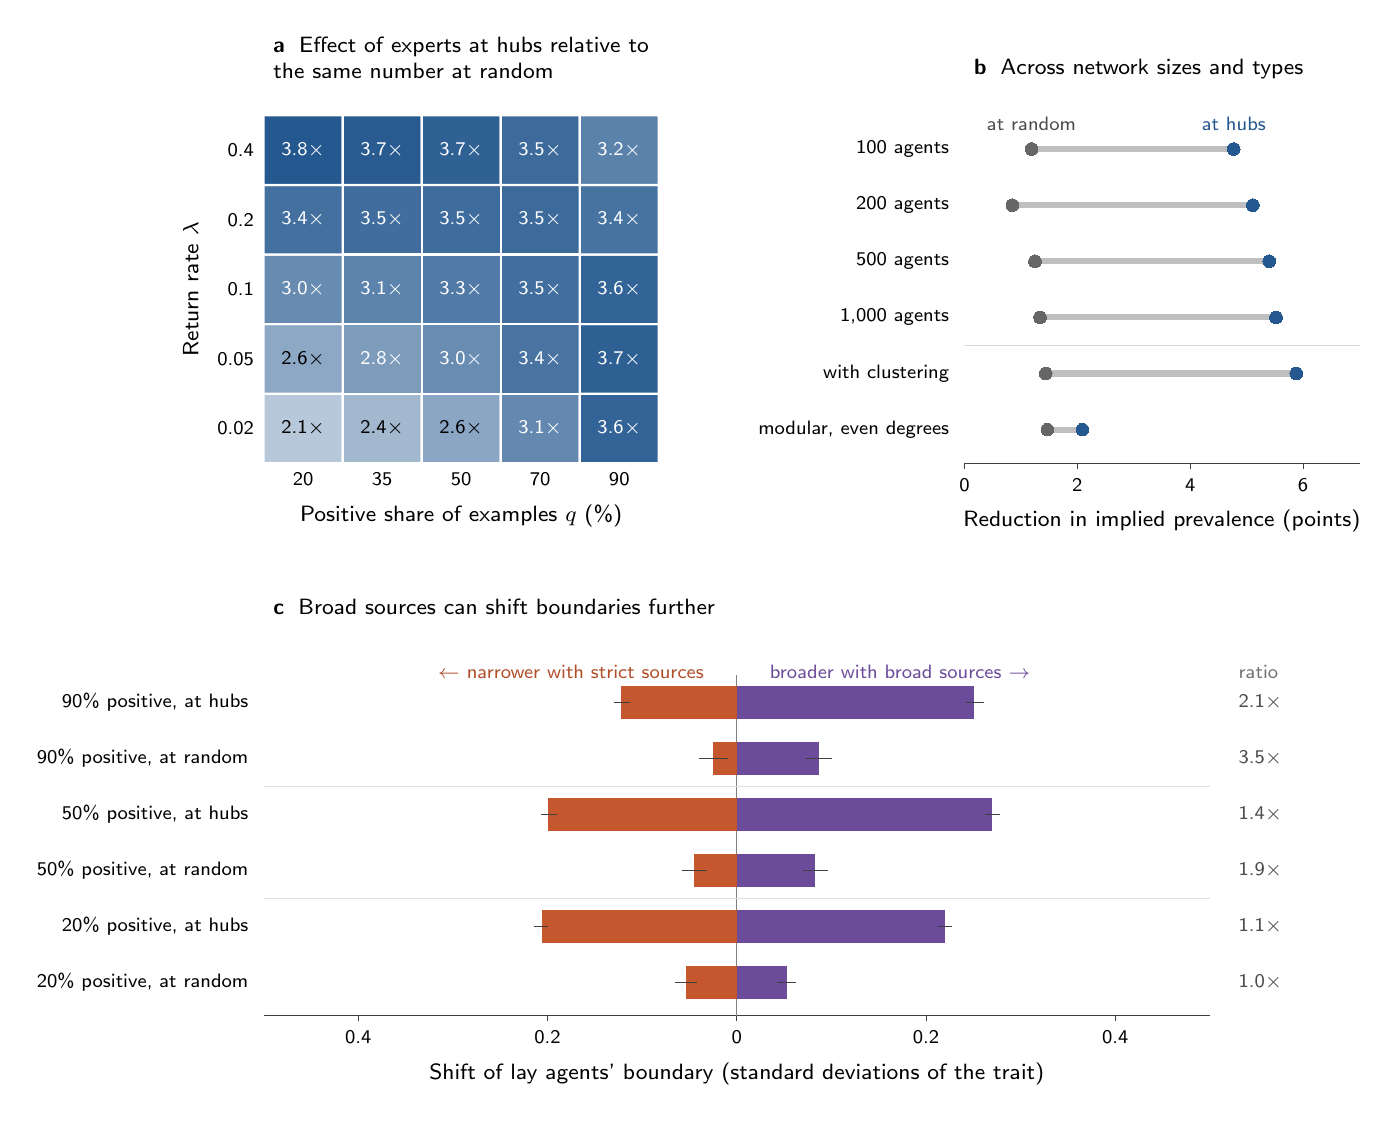
\begin{tikzpicture}[font=\sffamily\footnotesize]
\begin{axis}[pub,axis lines=box,width=6.6cm,height=6.0cm,title={\textbf{a}\hspace{0.6em}Effect of experts at hubs relative to\\the same number at random},xlabel={Positive share of examples $q$ (\%)},ylabel={Return rate $\lambda$},xmin=0.5,xmax=5.5,ymin=0.5,ymax=5.5,xtick={1,...,5},ytick={1,...,5},xticklabels={20,35,50,70,90},yticklabels={0.02,0.05,0.1,0.2,0.4},major tick length=0pt,colormap={seq}{color=(cA!8!white) color=(cA)},point meta min=1.5,point meta max=3.80,title style={text width=6cm}]
\addplot[matrix plot*,mesh/cols=5,mesh/rows=5,point meta=explicit,draw=white,line width=0.8pt] coordinates {(1,1) [2.120] (2,1) [2.358] (3,1) [2.618] (4,1) [3.064] (5,1) [3.617] (1,2) [2.590] (2,2) [2.780] (3,2) [3.005] (4,2) [3.368] (5,2) [3.670] (1,3) [3.028] (2,3) [3.146] (3,3) [3.276] (4,3) [3.454] (5,3) [3.609] (1,4) [3.421] (2,4) [3.471] (3,4) [3.486] (4,4) [3.512] (5,4) [3.387] (1,5) [3.797] (2,5) [3.732] (3,5) [3.655] (4,5) [3.514] (5,5) [3.157]};
\addplot[only marks,mark=none,point meta=explicit symbolic,nodes near coords,nodes near coords align={center},every node near coord/.append style={font=\sffamily\scriptsize,text=white,inner sep=0pt}] coordinates {(4,1) [3.1$\times$] (5,1) [3.6$\times$] (2,2) [2.8$\times$] (3,2) [3.0$\times$] (4,2) [3.4$\times$] (5,2) [3.7$\times$] (1,3) [3.0$\times$] (2,3) [3.1$\times$] (3,3) [3.3$\times$] (4,3) [3.5$\times$] (5,3) [3.6$\times$] (1,4) [3.4$\times$] (2,4) [3.5$\times$] (3,4) [3.5$\times$] (4,4) [3.5$\times$] (5,4) [3.4$\times$] (1,5) [3.8$\times$] (2,5) [3.7$\times$] (3,5) [3.7$\times$] (4,5) [3.5$\times$] (5,5) [3.2$\times$]};
\addplot[only marks,mark=none,point meta=explicit symbolic,nodes near coords,nodes near coords align={center},every node near coord/.append style={font=\sffamily\scriptsize,text=black,inner sep=0pt}] coordinates {(1,1) [2.1$\times$] (2,1) [2.4$\times$] (3,1) [2.6$\times$] (1,2) [2.6$\times$]};
\end{axis}
\begin{axis}[pub,at={(8.9cm,0cm)},width=6.6cm,height=6.0cm,title={\textbf{b}\hspace{0.6em}Across network sizes and types},xlabel={Reduction in implied prevalence (points)},xmin=0,xmax=7,ymin=0.4,ymax=6.6,ytick={1,...,6},yticklabels={{modular, even degrees},{with clustering},{1{,}000 agents},{500 agents},{200 agents},{100 agents}},y axis line style={draw=none},ytick style={draw=none}]
\draw[black!15,line width=0.4pt] (axis cs:0,2.5) -- (axis cs:7,2.5);
\draw[black!25,line width=2.2pt] (axis cs:1.47,1) -- (axis cs:2.09,1);
\addplot[only marks,mark=*,mark size=2.3pt,black!60,line width=0pt] coordinates {(1.47,1)};
\addplot[only marks,mark=*,mark size=2.3pt,cA,line width=0pt] coordinates {(2.09,1)};
\draw[black!25,line width=2.2pt] (axis cs:1.44,2) -- (axis cs:5.88,2);
\addplot[only marks,mark=*,mark size=2.3pt,black!60,line width=0pt] coordinates {(1.44,2)};
\addplot[only marks,mark=*,mark size=2.3pt,cA,line width=0pt] coordinates {(5.88,2)};
\draw[black!25,line width=2.2pt] (axis cs:1.34,3) -- (axis cs:5.52,3);
\addplot[only marks,mark=*,mark size=2.3pt,black!60,line width=0pt] coordinates {(1.34,3)};
\addplot[only marks,mark=*,mark size=2.3pt,cA,line width=0pt] coordinates {(5.52,3)};
\draw[black!25,line width=2.2pt] (axis cs:1.25,4) -- (axis cs:5.40,4);
\addplot[only marks,mark=*,mark size=2.3pt,black!60,line width=0pt] coordinates {(1.25,4)};
\addplot[only marks,mark=*,mark size=2.3pt,cA,line width=0pt] coordinates {(5.40,4)};
\draw[black!25,line width=2.2pt] (axis cs:0.85,5) -- (axis cs:5.11,5);
\addplot[only marks,mark=*,mark size=2.3pt,black!60,line width=0pt] coordinates {(0.85,5)};
\addplot[only marks,mark=*,mark size=2.3pt,cA,line width=0pt] coordinates {(5.11,5)};
\draw[black!25,line width=2.2pt] (axis cs:1.19,6) -- (axis cs:4.77,6);
\addplot[only marks,mark=*,mark size=2.3pt,black!60,line width=0pt] coordinates {(1.19,6)};
\addplot[only marks,mark=*,mark size=2.3pt,cA,line width=0pt] coordinates {(4.77,6)};
\node[font=\sffamily\scriptsize,text=black!70,anchor=south,inner sep=1.5pt] at (axis cs:1.1871343934250684,6.25) {at random};
\node[font=\sffamily\scriptsize,text=cA,anchor=south,inner sep=1.5pt] at (axis cs:4.771933372194686,6.25) {at hubs};
\end{axis}
\begin{axis}[pub,at={(0cm,-2.4cm)},anchor=north west,width=13.6cm,height=6.2cm,title={\textbf{c}\hspace{0.6em}Broad sources can shift boundaries further},xlabel={Shift of lay agents' boundary (standard deviations of the trait)},xmin=-0.5,xmax=0.5,ymin=0.4,ymax=6.9,ytick={1,...,6},yticklabels={{20\% positive, at random},{20\% positive, at hubs},{50\% positive, at random},{50\% positive, at hubs},{90\% positive, at random},{90\% positive, at hubs}},y axis line style={draw=none},ytick style={draw=none},xtick={-0.4,-0.2,0,0.2,0.4},xticklabels={0.4,0.2,0,0.2,0.4}]
\draw[black!50,line width=0.5pt] (axis cs:0,0.4) -- (axis cs:0,6.5);
\fill[cB] (axis cs:-0.054,0.7) rectangle (axis cs:0,1.3);
\fill[cD] (axis cs:0,0.7) rectangle (axis cs:0.053,1.3);
\draw[black!75,line width=0.5pt] (axis cs:-0.042,1) -- (axis cs:-0.065,1);
\draw[black!75,line width=0.5pt] (axis cs:0.042,1) -- (axis cs:0.063,1);
\node[font=\sffamily\scriptsize,anchor=west,text=black!70] at (axis cs:0.52,1) {1.0$\times$};
\fill[cB] (axis cs:-0.206,1.7) rectangle (axis cs:0,2.3);
\fill[cD] (axis cs:0,1.7) rectangle (axis cs:0.220,2.3);
\draw[black!75,line width=0.5pt] (axis cs:-0.199,2) -- (axis cs:-0.214,2);
\draw[black!75,line width=0.5pt] (axis cs:0.213,2) -- (axis cs:0.227,2);
\node[font=\sffamily\scriptsize,anchor=west,text=black!70] at (axis cs:0.52,2) {1.1$\times$};
\draw[black!12,line width=0.4pt] (axis cs:-0.5,2.5) -- (axis cs:0.5,2.5);
\fill[cB] (axis cs:-0.045,2.7) rectangle (axis cs:0,3.3);
\fill[cD] (axis cs:0,2.7) rectangle (axis cs:0.083,3.3);
\draw[black!75,line width=0.5pt] (axis cs:-0.031,3) -- (axis cs:-0.058,3);
\draw[black!75,line width=0.5pt] (axis cs:0.070,3) -- (axis cs:0.096,3);
\node[font=\sffamily\scriptsize,anchor=west,text=black!70] at (axis cs:0.52,3) {1.9$\times$};
\fill[cB] (axis cs:-0.199,3.7) rectangle (axis cs:0,4.3);
\fill[cD] (axis cs:0,3.7) rectangle (axis cs:0.270,4.3);
\draw[black!75,line width=0.5pt] (axis cs:-0.190,4) -- (axis cs:-0.207,4);
\draw[black!75,line width=0.5pt] (axis cs:0.262,4) -- (axis cs:0.278,4);
\node[font=\sffamily\scriptsize,anchor=west,text=black!70] at (axis cs:0.52,4) {1.4$\times$};
\draw[black!12,line width=0.4pt] (axis cs:-0.5,4.5) -- (axis cs:0.5,4.5);
\fill[cB] (axis cs:-0.025,4.7) rectangle (axis cs:0,5.3);
\fill[cD] (axis cs:0,4.7) rectangle (axis cs:0.087,5.3);
\draw[black!75,line width=0.5pt] (axis cs:-0.009,5) -- (axis cs:-0.040,5);
\draw[black!75,line width=0.5pt] (axis cs:0.072,5) -- (axis cs:0.101,5);
\node[font=\sffamily\scriptsize,anchor=west,text=black!70] at (axis cs:0.52,5) {3.5$\times$};
\fill[cB] (axis cs:-0.122,5.7) rectangle (axis cs:0,6.3);
\fill[cD] (axis cs:0,5.7) rectangle (axis cs:0.251,6.3);
\draw[black!75,line width=0.5pt] (axis cs:-0.113,6) -- (axis cs:-0.130,6);
\draw[black!75,line width=0.5pt] (axis cs:0.242,6) -- (axis cs:0.261,6);
\node[font=\sffamily\scriptsize,anchor=west,text=black!70] at (axis cs:0.52,6) {2.1$\times$};
\node[font=\sffamily\scriptsize,text=cB!90!black,anchor=east,inner sep=1.5pt] at (axis cs:-0.03,6.55) {$\leftarrow$ narrower with strict sources};
\node[font=\sffamily\scriptsize,text=cD,anchor=west,inner sep=1.5pt] at (axis cs:0.03,6.55) {broader with broad sources $\rightarrow$};
\node[font=\sffamily\scriptsize,anchor=west,text=black!55] at (axis cs:0.52,6.55) {ratio};
\end{axis}
\end{tikzpicture}}

\newcommand{\figpred}{%
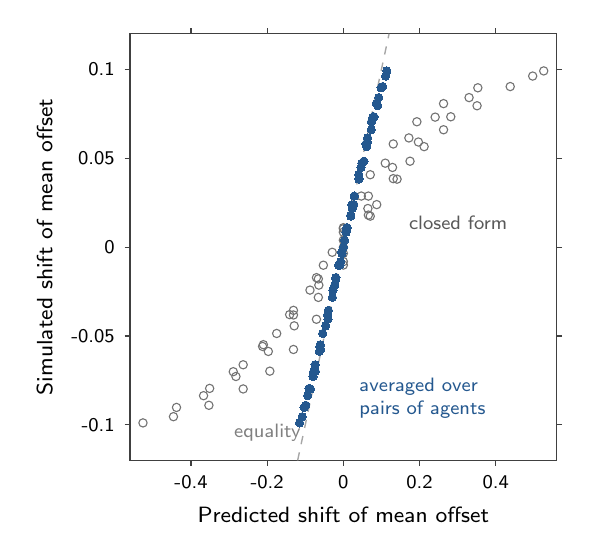
\begin{tikzpicture}[font=\sffamily\footnotesize]
\begin{axis}[pub,axis lines=box,width=7cm,height=7cm,xlabel={Predicted shift of mean offset},ylabel={Simulated shift of mean offset},xmin=-0.56,xmax=0.56,ymin=-0.12,ymax=0.12,scaled ticks=false,tick label style={font=\sffamily\scriptsize,/pgf/number format/fixed},clip=true]
\addplot[black!35,dashed,domain=-0.12:0.12,samples=2,line width=0.5pt] {x};
\addplot[only marks,mark=o,mark size=1.5pt,black!55,line width=0.4pt] coordinates {(0,0.0103) (0.0262,0.0237) (0.0706,0.0407) (0.131,0.058) (0.193,0.0705) (0.263,0.0807) (0.353,0.0896) (0.526,0.0991) (-0.0292,-0.00293) (0,0.0109) (0.0471,0.0287) (0.11,0.0472) (0.172,0.0614) (0.241,0.0731) (0.33,0.0841) (0.497,0.0962) (-0.0876,-0.0242) (-0.0525,-0.0102) (0,0.00839) (0.0657,0.0287) (0.129,0.0448) (0.197,0.0591) (0.282,0.0733) (0.438,0.0903) (-0.175,-0.0486) (-0.131,-0.0356) (-0.0706,-0.0172) (0,0.00387) (0.0644,0.0217) (0.131,0.0385) (0.212,0.0565) (0.351,0.0795) (-0.263,-0.0662) (-0.21,-0.0549) (-0.141,-0.038) (-0.0657,-0.0179) (0,-0.000153) (0.0657,0.018) (0.141,0.0382) (0.263,0.066) (-0.351,-0.0795) (-0.289,-0.0701) (-0.212,-0.0559) (-0.131,-0.0382) (-0.0644,-0.0214) (0,-0.00354) (0.0706,0.0174) (0.175,0.0483) (-0.438,-0.0902) (-0.367,-0.0836) (-0.282,-0.0728) (-0.197,-0.0587) (-0.129,-0.0443) (-0.0657,-0.0283) (0,-0.00817) (0.0876,0.0239) (-0.526,-0.0989) (-0.446,-0.0954) (-0.353,-0.089) (-0.263,-0.0798) (-0.193,-0.0698) (-0.131,-0.0576) (-0.0706,-0.0406) (0,-0.0101)};
\addplot[only marks,mark=*,mark size=1.5pt,cA,line width=0pt] coordinates {(0.009,0.0103) (0.0221,0.0237) (0.0405,0.0407) (0.0594,0.058) (0.0737,0.0705) (0.0863,0.0807) (0.0992,0.0896) (0.114,0.0991) (-0.00464,-0.00293) (0.00969,0.0109) (0.0288,0.0287) (0.0485,0.0472) (0.0636,0.0614) (0.0775,0.0731) (0.0928,0.0841) (0.111,0.0962) (-0.0274,-0.0242) (-0.0126,-0.0102) (0.00719,0.00839) (0.0287,0.0287) (0.0464,0.0448) (0.063,0.0591) (0.0804,0.0733) (0.103,0.0903) (-0.0543,-0.0486) (-0.0394,-0.0356) (-0.0195,-0.0172) (0.00339,0.00387) (0.0232,0.0217) (0.0408,0.0385) (0.0613,0.0565) (0.0902,0.0795) (-0.0742,-0.0662) (-0.0605,-0.0549) (-0.0411,-0.038) (-0.0198,-0.0179) (0.000175,-0.000153) (0.0196,0.018) (0.041,0.0382) (0.0732,0.066) (-0.09,-0.0795) (-0.0782,-0.0701) (-0.0617,-0.0559) (-0.0415,-0.0382) (-0.0226,-0.0214) (-0.00359,-0.00354) (0.0196,0.0174) (0.0541,0.0483) (-0.103,-0.0902) (-0.0938,-0.0836) (-0.0795,-0.0728) (-0.0628,-0.0587) (-0.0464,-0.0443) (-0.0288,-0.0283) (-0.00702,-0.00817) (0.0274,0.0239) (-0.115,-0.0989) (-0.108,-0.0954) (-0.0985,-0.089) (-0.0864,-0.0798) (-0.0737,-0.0698) (-0.0594,-0.0576) (-0.0404,-0.0406) (-0.00876,-0.0101)};
\node[font=\sffamily\scriptsize,text=cA,anchor=west,inner sep=1.5pt,align=left] at (axis cs:0.03,-0.085) {averaged over\\pairs of agents};
\node[font=\sffamily\scriptsize,text=black!65,anchor=north west,inner sep=1.5pt] at (axis cs:0.16,0.02) {closed form};
\node[font=\sffamily\scriptsize,text=black!50,anchor=south east,inner sep=1.5pt] at (axis cs:-0.1,-0.112) {equality};
\end{axis}
\end{tikzpicture}}

\newcommand{\figprofile}{%
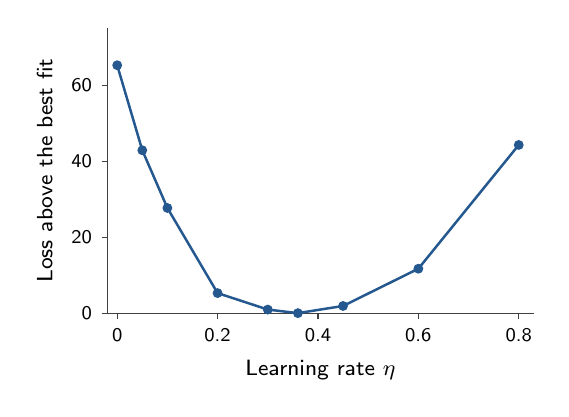
\begin{tikzpicture}[font=\sffamily\footnotesize]
\begin{axis}[pub,width=7cm,height=5.2cm,xlabel={Learning rate $\eta$},ylabel={Loss above the best fit},ymin=0,ymax=75.05,xmin=-0.02,xmax=0.83]
\addplot[cA,mark=*,mark size=1.3pt] coordinates {(0,65.3) (0.05,42.9) (0.1,27.7) (0.2,5.28) (0.3,0.937) (0.36,0) (0.45,1.89) (0.6,11.7) (0.8,44.3)};
\end{axis}
\end{tikzpicture}}
\newcommand{\figconcept}{%
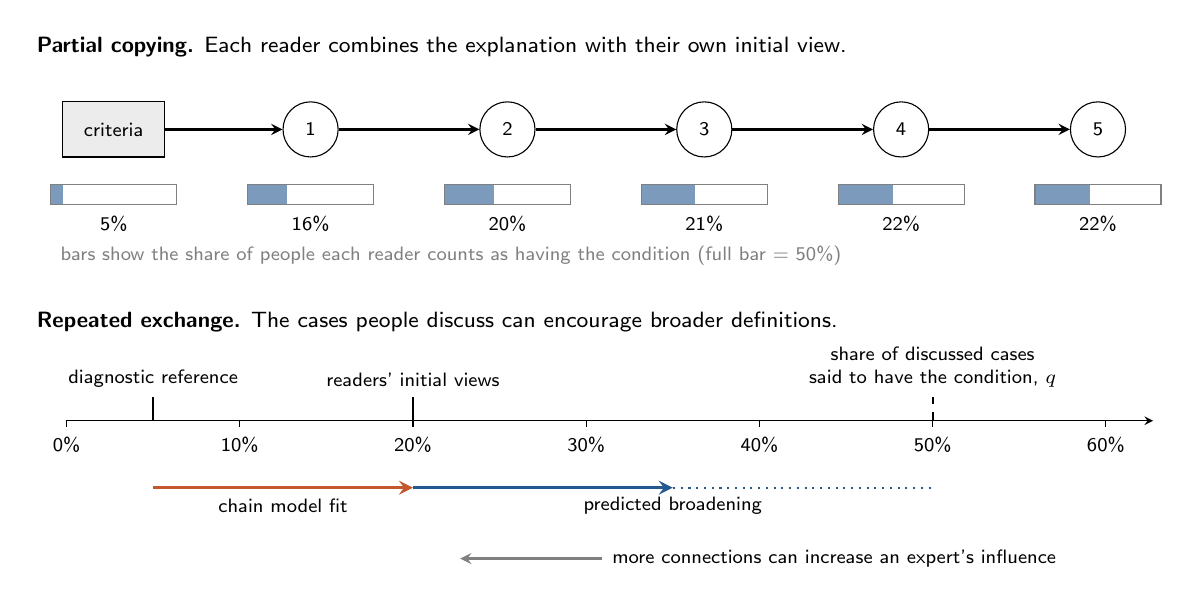
\begin{tikzpicture}[font=\sffamily\scriptsize,>=stealth]
\node[anchor=west,font=\sffamily\footnotesize] at (0,4.75) {\textbf{Partial copying.} Each reader combines the explanation with their own initial view.};
\node[draw,fill=gray!15,minimum width=1.3cm,minimum height=0.7cm] (p0) at (1.1,3.7) {criteria};
\foreach \i/\x/\w/\l in {0/1.1/0.10/5,1/3.6/0.31528/16,2/6.1/0.39537/20,3/8.6/0.42302/21,4/11.1/0.43457/22,5/13.6/0.43860/22} {
  \fill[cA!60] (\x-0.8,2.75) rectangle (\x-0.8+1.6*\w,3.0);
  \draw[gray] (\x-0.8,2.75) rectangle (\x+0.8,3.0);
  \node at (\x,2.5) {\l\%};
}
\foreach \i/\x in {1/3.6,2/6.1,3/8.6,4/11.1,5/13.6} {\node[circle,draw,minimum size=0.7cm] (p\i) at (\x,3.7) {\i};}
\foreach \a/\b in {0/1,1/2,2/3,3/4,4/5} {\draw[->,thick] (p\a) -- (p\b);}
\node[anchor=west,text=gray] at (0.3,2.1) {bars show the share of people each reader counts as having the condition (full bar = 50\%)};
\node[anchor=west,font=\sffamily\footnotesize] at (0,1.25) {\textbf{Repeated exchange.} The cases people discuss can encourage broader definitions.};
\draw[->] (0.5,0) -- (14.3,0);
\foreach \p in {0,10,20,30,40,50,60} {\draw (0.5+0.22*\p,0) -- (0.5+0.22*\p,-0.08) node[below] {\p\%};}
\draw[thick] (1.6,0) -- (1.6,0.3) node[above] {diagnostic reference};
\draw[thick] (4.9,0) -- (4.9,0.3) node[above] {readers' initial views};
\draw[thick,dashed] (11.5,0) -- (11.5,0.3) node[above,align=center] {share of discussed cases\\said to have the condition, $q$};
\draw[->,very thick,cB] (1.6,-0.85) -- (4.9,-0.85) node[midway,below,text=black] {chain model fit};
\draw[->,very thick,cA] (4.9,-0.85) -- (8.2,-0.85);
\draw[cA,thick,dotted] (8.2,-0.85) -- (11.5,-0.85);
\node[below] at (8.2,-0.85) {predicted broadening};
\draw[<-,thick,gray] (5.5,-1.75) -- (7.3,-1.75) node[right,text=black] {more connections can increase an expert's influence};
\end{tikzpicture}}
\newcommand{\figlearningrules}{%
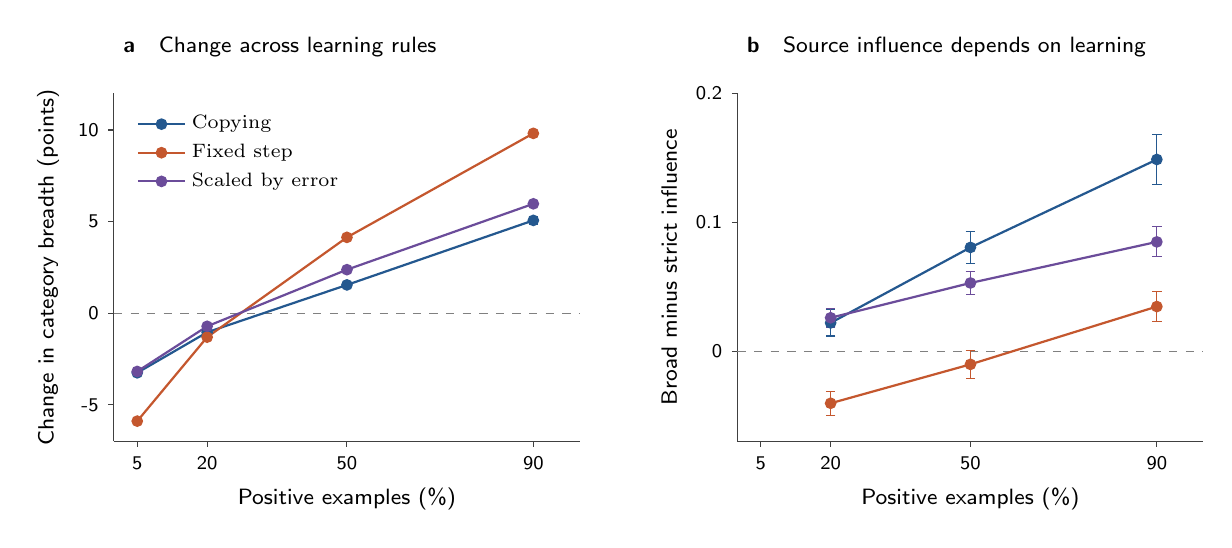
\begin{tikzpicture}[font=\sffamily\footnotesize]
\begin{groupplot}[pub,group style={group size=2 by 1,horizontal sep=2.0cm},width=7.5cm,height=6.0cm,xlabel={Positive examples (\%)},xmin=0,xmax=100,xtick={5,20,50,90},legend style={draw=none,fill=none,font=\scriptsize}]
\nextgroupplot[title={\textbf{a}\quad Change across learning rules},ylabel={Change in category breadth (points)},ymin=-7,ymax=12,legend style={at={(0.03,0.97)},anchor=north west}]
\draw[gray,dashed] (axis cs:0,0)--(axis cs:100,0);
\addplot[cA,thick,mark=*,mark size=1.7pt,error bars/.cd,y dir=both,y explicit] coordinates {(5,-3.25930) +- (0,0.09322) (20,-1.04705) +- (0,0.04712) (50,1.54101) +- (0,0.04173) (90,5.06413) +- (0,0.19776) };
\addplot[cB,thick,mark=*,mark size=1.7pt,error bars/.cd,y dir=both,y explicit] coordinates {(5,-5.89838) +- (0,0.09134) (20,-1.31267) +- (0,0.05808) (50,4.13745) +- (0,0.05397) (90,9.81696) +- (0,0.11881) };
\addplot[cD,thick,mark=*,mark size=1.7pt,error bars/.cd,y dir=both,y explicit] coordinates {(5,-3.18556) +- (0,0.07184) (20,-0.71956) +- (0,0.03910) (50,2.37298) +- (0,0.04687) (90,5.96933) +- (0,0.13158) };
\legend{Copying,Fixed step,Scaled by error}
\nextgroupplot[title={\textbf{b}\quad Source influence depends on learning},ylabel={Broad minus strict influence},ymin=-0.07,ymax=0.2]
\draw[gray,dashed] (axis cs:0,0)--(axis cs:100,0);
\addplot[cA,thick,mark=*,mark size=1.7pt,error bars/.cd,y dir=both,y explicit] coordinates {(20,0.02188) +- (0,0.01013) (50,0.08045) +- (0,0.01219) (90,0.14871) +- (0,0.01920) };
\addplot[cB,thick,mark=*,mark size=1.7pt,error bars/.cd,y dir=both,y explicit] coordinates {(20,-0.04049) +- (0,0.00929) (50,-0.01029) +- (0,0.01078) (90,0.03457) +- (0,0.01192) };
\addplot[cD,thick,mark=*,mark size=1.7pt,error bars/.cd,y dir=both,y explicit] coordinates {(20,0.02586) +- (0,0.00719) (50,0.05287) +- (0,0.00915) (90,0.08476) +- (0,0.01168) };
\end{groupplot}
\end{tikzpicture}}

\newcommand{\todo}[1]{\textcolor{red}{[#1]}}

\title{Partial copying and the broadening of diagnostic categories through peer transmission}
\author{Kyuri Park$^{1}$\\[2pt]
{\small $^{1}$Computational Science Lab, Informatics Institute, University of Amsterdam}}
\date{}

\begin{document}
\maketitle

\begin{abstract}
\noindent How does passing on an explanation of a diagnosis change who people think has it? We study a model in which people begin with their own understanding of a condition and partly adopt another person's view when they disagree about a case. The model reproduces the gradual broadening observed when explanations of ADHD were passed along a chain of readers. The data cannot establish that this learning process caused the change, because differences between the groups tested on different days could also account for the pattern. In simulations of repeated discussion, talking mainly about people described as having the condition can encourage broader definitions. Broad descriptions can then have more influence than strict ones. These predictions depend on which cases people discuss and require tests beyond the transmission experiment.
\end{abstract}

\section{Introduction}

People learn what a diagnosis means from explanations given by other people as well as from clinical criteria. These explanations can differ in who they seem to include. Two readers may agree that someone has difficulty concentrating yet disagree about whether that person has ADHD. If they pass on their own explanations, will these differences simply make the meaning less precise, or can they gradually change who is thought to have the condition?

This question concerns the breadth of a diagnosis, meaning the range of people to whom it is applied. Haslam describes the widening of concepts of harm and pathology as \emph{concept creep} \citep{haslam2016}. Foulkes and Andrews propose that mental-health awareness efforts may contribute to this process by leading people to interpret milder distress as a disorder \citep{foulkes2023}. Here we examine a possible learning process behind such broadening. A person may take in part of an explanation while retaining some of their own understanding, and then pass this combined view to someone else.

A recent experiment provides a way to examine this idea. \citet{katiyar2026} passed explanations of ADHD from one participant to the next, following a design used to study how information changes through transmission \citep{bartlett1932,mesoudi2008}. The first participant read the DSM-5-TR criteria \citep{dsm5tr} and wrote an explanation for another participant. Each later participant read the previous explanation and wrote a new one. In the main study, participants further along the chains were more likely to say that a fictional person with symptoms below the diagnostic threshold had ADHD. This is consistent with a diagnosis being applied more broadly as explanations are passed on. It leaves open how the change arose and whether the same process would operate when people learn from one another repeatedly.

We model this process by giving each person an initial understanding of who has the condition. They encounter examples of people described as having it and people described as not having it. When they disagree with the person supplying an example, they partly adjust their own judgement towards that person's view. We call this \emph{partial copying}. In a chain of readers, each new person brings their own understanding to what they read. An initially strict explanation can therefore become broader as it passes through people whose existing views are broader. When the same people exchange examples repeatedly, a further question arises. Does it matter how often they discuss people said to have the condition, compared with people said not to have it?

Previous research gives reasons to expect both learning from others and the selection of examples to matter. Models and experiments show how people can come to use the same words or categories by adjusting to one another after disagreements \citep{steels1995,baronchelli2006,puglisi2008,centola2015}. Judgements also depend on which examples people encounter \citep{parducci1965,levari2018}. Work on information passed through successive learners shows how their existing expectations can shape what is transmitted \citep{griffiths2007,kalish2007}. 

We examine two settings. First, we fit the model to the ADHD experiment to ask whether partial copying can account for the changes along the chains. We compare it with explanations that do not require each reader to inherit the previous reader's understanding. This matters because each round of the experiment used a different group of participants tested on a different day. Second, we simulate repeated exchanges within networks, where people can learn from several others and may encounter stricter sources whose views do not change. Earlier models show that people who keep their views fixed can influence a much larger group, and that their position in the network affects their reach \citep{mobilia2003,mobilia2007,xie2011,centola2018,acemoglu2013,yildiz2013,hunter2022}. We compare the influence of broad and strict descriptions and ask whether well-connected experts can limit broadening. The chain experiment helps us fit the learning model, but it does not test these predictions about repeated discussion. Figure~\ref{fig:concept} shows the distinction.

\begin{figure}[tbp]
\centering
\resizebox{\textwidth}{!}{\figconcept}
\caption{One reading and repeated discussion. In the upper panel, each person reads one explanation and passes on a version shaped by their own initial understanding. The percentages show how many people each reader would classify as having the condition in the fitted model. The readers' initial views were estimated from their later responses, not measured before reading. The lower panel shows what the model predicts when people exchange examples repeatedly. Discussing many people said to have the condition can broaden its use further. Here $q$ is the share of discussed cases described as having the condition. The population need not reach that share, because change can stop when people agree or be limited by a return towards their initial views.}
\label{fig:concept}
\end{figure}

\section{Results}

\subsection{Model}

In the model, a learner's understanding of ADHD determines which cases they classify as having it. We represent a case by a person's levels of inattention and hyperactivity, and the learner's judgement by a line separating cases they include from those they exclude. We call this line the \emph{category boundary}. A broader definition classifies more people as having the condition, while a stricter definition classifies fewer.

Formally, a case is a point $x \in \mathbb{R}^2$, with coordinates representing inattention and hyperactivity, and $x \sim \mathcal{N}(0, I)$. Each learner uses a linear boundary with angle $\phi$ and offset $b$, and classifies $x$ as having the condition when $u(\phi)^\top x > b$, where $u(\phi) = (\cos\phi, \sin\phi)$. The learner's category therefore covers a share $\pi(b) = 1 - \Phi(b)$ of people, where $\Phi$ is the standard normal distribution function. The diagnostic boundary is fixed at $\phi_D = \pi/4$ and $b_D = \Phi^{-1}(0.95)$, which corresponds to a share of 5\%. This is an imposed reference within the model, not an estimate of clinical ADHD prevalence or a formal representation of the full DSM criteria. We use \emph{implied prevalence} to mean the fraction classified positive by a model boundary.

A learner receives ten examples from another person, whom we call the source. The source labels each case as having the condition (a positive example) or not having it (a counter-example). We use $n=10$ for the number of examples per reading. Positive cases are sampled from the population conditional on lying on the source's positive side, and counter-examples from the other side. In network simulations, each example is independently positive with probability $q$. On every example where the reader's own label differs from the source's, the reader moves toward the source,
\begin{equation}
(\phi, b) \leftarrow (\phi, b) + \eta \, \bigl[(\phi_S, b_S) - (\phi, b)\bigr],
\label{eq:update}
\end{equation}
where $0 \leq \eta \leq 1$ is the fraction of the remaining parameter difference copied at each disagreement. Examples on which the two agree leave the reader unchanged. Thus $\eta$ is not the fraction copied over an entire reading of ten examples. The rule assumes that disagreement permits movement toward the source's boundary, an abstraction of learning rather than an inference algorithm that reconstructs a boundary from labels alone.

We use the rule in two settings. In a chain, each new learner starts from their own initial boundary, which we call the lay prior, with $b \sim \mathcal{N}(\mu_b, s_b^2)$ and $\phi \sim \mathcal{N}(\pi/4, (15^\circ)^2)$, and reads once, from the diagnostic boundary at generation~1 and from its predecessor afterwards. In a population, agents read repeatedly from their network neighbours and, after each reading, move a fraction $\lambda$ of the way back to their own prior. To connect the model to data, we treat responses as noisy readings of the boundary. Reported prevalence satisfies $\operatorname{logit}(\text{report}) = \operatorname{logit}\pi(b) + \varepsilon_p$. A vignette character is a point $x_V = (v, v)$ and is diagnosed when $u^\top x_V - b + \varepsilon_r > 0$. Self-diagnosis uses the agent's own position $x_s \sim \mathcal{N}(0, I)$ and an offset $c_s$, with a positive response when $u^\top x_s - b + c_s + \varepsilon_r > 0$. The noise terms are normal with standard deviations $\sigma_p$ and $\sigma_r$.

\subsection{Repeated exchange has a direction}
\label{sec:drift}

When agents read one another repeatedly, update rule~\eqref{eq:update} moves the population's boundaries in a predictable direction. The reason is that the two kinds of example correct different readers (Figure~\ref{fig:drift}a). When boundaries have the same orientation and categories are nested, a positive case can only correct a stricter reader, and a counter-example can only correct a broader reader. With different orientations, categories need not be nested and this one-dimensional argument is only an approximation. How often each correction happens depends on how rare the category is.

Consider two agents with the same orientation and offsets $b_1 < b_2$, so that agent~1 holds the broader category, and let $G = \Phi(b_2) - \Phi(b_1)$ be the share of people on whom they disagree. When the stricter agent reads the broader one, it is corrected by positive cases that fall in the gap, and a positive case from agent~1 falls there with probability $G / [1 - \Phi(b_1)]$. When the broader agent reads the stricter one, it is corrected by counter-examples in the gap, each of which falls there with probability $G / \Phi(b_2)$. Every correction moves the reader by $\eta (b_2 - b_1)$ toward the other agent. With a common share $q$ of positive cases and equally likely reading directions, the expected change in the pair's mean offset per example exchanged is proportional to
\begin{equation}
\frac{1-q}{\Phi(b_2)} - \frac{q}{1 - \Phi(b_1)}
\;\longrightarrow\;
\frac{\pi - q}{\pi (1 - \pi)}
\quad \text{as } b_1, b_2 \to b, \; \pi = 1 - \Phi(b).
\label{eq:drift}
\end{equation}
In this local limit, the mean offset increases when $\pi > q$ and decreases when $\pi < q$, favouring narrowing and broadening respectively. For a finite gap the exact balance occurs at $q_* = [1-\Phi(b_1)]/[\Phi(b_2)+1-\Phi(b_1)]$, rather than generally at either agent's prevalence. The local sign rule describes a direction of change while disagreement persists, not a guarantee of convergence to prevalence $q$.

For a rare category, even a minority of positive examples can favour broadening in the local approximation. For boundaries implying prevalence between 5\% and 20\%, this approximation predicts broadening when more than a fifth of the exchanged cases are positive. Whether everyday ADHD communication meets this condition is an empirical question. The factor $1/[\pi(1-\pi)]$ shows why rarity matters. Positive cases of a rare category are concentrated just above the boundary, where a stricter reader disagrees, whereas counter-examples are spread over almost the whole population and seldom fall where a broader reader disagrees. In the example of Figure~\ref{fig:drift}a, 58\% of the source's positive cases correct the stricter reader, but only 18\% of its counter-examples correct the broader one.

\begin{figure}[tbp]
\centering
\resizebox{\textwidth}{!}{\figasym}
\caption{Direction of drift under repeated exchange. (a) A source with a rare category corrects a stricter reader through positive cases in the orange region and a broader reader through counter-examples in the blue region. (b) Simulated shift of the mean boundary after one round of exchange, for populations with different prevalence at their mean initial offset and different shares of positive cases. Blue indicates broadening and orange narrowing. The dashed line marks $\pi = q$, where the local approximation predicts no drift. Finite heterogeneity can produce nonzero drift on this line. (c) Late-run implied prevalence in a population that starts from the baseline lay priors and reverts toward them at rate $\lambda$ per round.}
\label{fig:drift}
\end{figure}

Equation~\eqref{eq:drift} is derived for one pair with nearly equal boundaries. To check it in heterogeneous populations, we simulated one round of exchange for 64 combinations of category prevalence and positive share, using the parameter settings specified in Methods. The sign of the shift in the mean boundary matches the prediction in all 56 combinations with $\pi \neq q$ (Figure~\ref{fig:drift}b).

This direction of change does not require direct access to the source's boundary in the settings we tested. We repeated the one-round grid with aligned boundaries and two label-only learners. One moves its offset by a fixed step after each misclassified example. The other moves a fraction $\eta$ of the way toward that example's position along the common boundary normal. Both match the local sign prediction in all 56 off-diagonal combinations (Methods). This check concerns one-dimensional, aligned boundaries and one round of exchange. It does not establish the same long-run behaviour for general boundary-learning rules.

A leading-order approximation also predicts the size of the shift. For aligned boundaries with small offset differences and negligible change in those differences within a reading, the expected change in the mean offset over one round is $n \eta s_b^2 \varphi(b) (\pi - q) / [\pi (1 - \pi)]$, where $\varphi$ is the standard normal density. This expression closely tracks the ordering of the 64 combinations (correlation 0.97 with the simulated shifts) but overstates their size about fourfold at the estimated heterogeneity, consistent with corrections within a reading narrowing the gap and reducing the chance of further corrections. Finite heterogeneity and orientation differences also lie outside the approximation. A deterministic mean-update approximation, averaged over pairs of aligned boundaries without sampling examples, tracks the simulated shifts closely (correlation 0.999, regression slope 0.91, Supplementary Figure~\ref{fig:pred}).

The size of the drift depends on how much disagreement remains. It stops once a population reaches consensus and can continue when newcomers or each person's pull back toward a prior belief keep boundaries apart. With the baseline priors, whose mean implied prevalence is about 21\%, and $\lambda = 0.02$, the simulations yield a late-run implied prevalence of 16\% when 5\% of examples are positive, 24\% when half are, and 30\% when nine in ten are (Figure~\ref{fig:drift}c). The spread of priors matters for these magnitudes. Holding the other main-fit parameters fixed and varying $s_b$ by one approximate standard error gives implied prevalence from 22\% to 25\% when half the examples are positive and from 25\% to 33\% when nine in ten are. This is a sensitivity analysis, not a confidence interval. Peer exchange can raise mean category breadth above its initial population average. It does not move offsets beyond the range of the initial and fixed source offsets, because each update and reversion is a convex combination. Neither $\lambda$ nor $q$ can be estimated from the chain data, so these magnitudes are conditional on their values.

\subsection{Partial copying describes broadening in transmission chains}
\label{sec:chain}

We calibrate the model on Study~3 of \citet{katiyar2026}. In each of 220 chains the first participant read the DSM-5-TR criteria for ADHD and wrote an explanation for the next participant, and each later participant read only the explanation written by the one before, for seven generations. After reading, participants judged whether a vignette character with subclinical symptoms (\textquotedblleft Vincent\textquotedblright) has ADHD, whether they themselves do, and what share of the population does (Methods).

\begin{figure}[tbp]
\centering
\resizebox{0.92\textwidth}{!}{\figmech}
\caption{The model fitted to the chain experiment. (a) Distribution of the share of people each reader counts as having ADHD, by generation, in the fitted model, with the lay prior that readers hold before reading at the bottom. One reading of the diagnostic criteria (5\%) leaves readers between the criteria and their prior, and from the third generation on the distribution is close to the prior. (b--d) Generation means of the three measures (adjusted, with 95\% intervals). Blue bands show the middle 50\% and 90\% of generation means across 400 simulated experiments of 220 chains under fixed fitted parameters, excluding parameter-estimation uncertainty. Orange dashed lines show the constant-source no-lineage alternative. Purple dotted lines show the changing-source alternative.}
\label{fig:mech}
\end{figure}

We estimate seven parameters by the method of simulated moments, using 31 moments of the data. These comprise the generation means of the three measures, the spread of prevalence estimates, and the correlation of each measure between successive participants in a chain (Methods). We first compare four versions of the model. Three are versions of partial copying that differ in whether the examples a lay text is assumed to carry are half positive, positive only, or sampled at the population base rate. The fourth has no lineage. From generation~2 on, every reader learns from one shared lay boundary, so that nothing specific to a chain is passed on. All versions use five positive examples followed by five counter-examples at generation~1. The half-positive and no-lineage versions retain this ordering in later generations. The positive-only version uses ten positive examples thereafter, and the base-rate version samples each label at the source's implied prevalence. Example order is therefore another modelling assumption.

\begin{table}[htbp]
\centering
\caption{Fit to Study~3 using 31 moments and adjusted means. Lower loss indicates a closer fit. Fit loss uses 3,000 simulated chains. The simulation check averages the same criterion over three new seeds with 20,000 chains each, at fixed fitted parameters. It uses the same observations as the fit. Partial-copying models have seven parameters, the constant-source alternative eight and the changing-source alternative nine. Lay prior is prevalence at the mean prior offset.}
\label{tab:fit}
\begingroup\small\setlength{\tabcolsep}{5pt}
\begin{tabular}{lrrrr}
\toprule
Model & Fit loss & Simulation check & $\eta$ & Lay prior (\%) \\
\midrule
Half positive & 32.9 & 32.6 & 0.31 & 20.2 \\
Positive only & 34.1 & 33.1 & 0.23 & 19.1 \\
Base rate & 29.8 & 30.3 & 0.35 & 21.4 \\
No lineage, constant source & 42.5 & 42.1 & -- & -- \\
No lineage, changing source & 27.8 & 29.4 & -- & -- \\
\bottomrule
\end{tabular}\endgroup
\end{table}

The partial-copying versions have lower in-sample loss than the constant-source no-lineage alternative (Table~\ref{tab:fit}, Figure~\ref{fig:mech}b--d). Without lineage, the model predicts a single jump at generation~2 followed by a plateau. The other-diagnosis and prevalence trajectories instead rise over several generations. Within this model comparison, partial inheritance captures that gradual change better. The comparison does not establish that inheritance is the only possible explanation. The three versions of partial copying give the same account. Lay readers start from a boundary that covers about 20\% of people. One reading moves them only part of the way toward the source, with $\eta$ between 0.23 and 0.35. The diagnostic boundary is therefore diluted at every step, and by the fourth generation the mean boundary is close to the lay prior (Figure~\ref{fig:mech}a). On this account, the broadening largely reflects relaxation toward an inferred lay prior. Participants' pre-exposure boundaries were not directly measured, so the fitted prior is a model-dependent explanation rather than an observed baseline.

Partial copying also has lower loss than the constant-source alternative when unadjusted generation means are fitted (37 against 54) and when participants flagged for possible AI use are removed together with everyone downstream of them in their chain. Recomputing all moments in the retained sample of 1{,}168 participants gives losses of 33 and 45. Leaving out generations 6 and 7, whose participants differed most from the rest, gives losses of 15.7 and 22.9 on 23 moments. Study~2, where the observed broadening is weaker, gives losses of 32 and 40. These comparisons retain their ordering with larger simulations at new seeds. The half-positive learning rate is estimated at 0.31 with an approximate standard error of 0.08, and prevalence at the mean lay prior at 20.2\% with a standard error of 0.7 percentage points. A descriptive profile on unadjusted means gives higher loss at zero learning and at the largest rate examined (Supplementary Figure~\ref{fig:profile}). Supplementary Tables~\ref{tab:params} and~\ref{tab:losses} report estimates and sensitivity fits.

The comparison changes when the shared lay source is allowed to change across generations. This no-lineage model has two more parameters than partial copying and gives lower loss, 27.8 against 32.9. Re-evaluation with larger simulations gives 29.4 against 32.6 (Table~\ref{tab:fit}). These are descriptive fitting losses, without a penalty for model complexity. They do not establish a preferred mechanism. They do show that the mean trajectory alone cannot separate inheritance along a chain from changes in a source shared by each generation. Because generations were collected on different days, such an alternative also represents a limitation of the experimental design.

We also generated ten synthetic experiments from each of the fitted half-positive and constant-source models and refitted both models to each (Supplementary Table~\ref{tab:recovery}). In the larger-simulation check, partial copying had lower loss in all ten datasets generated by partial copying. The constant-source model had lower loss in four of ten datasets generated without lineage. The largest loss gap favouring partial copying without lineage was 12.4, compared with 9.5 in the observed data under the same larger-simulation check. Refitting partial copying to its own synthetic data gave learning rates from 0.20 to 0.51, against a generating value of 0.31, while prevalence at the mean prior ranged from 19.1\% to 21.1\%. One of the constant-source comparisons was effectively tied, with a loss difference below 0.01. The check is conditional on the fitted generating parameters and the observed-data weights. It does not include the changing-source alternative or reproduce uncertainty from covariate adjustment. Ten experiments per generating model are insufficient to establish reliable model selection across the parameter space.

Two features of the mechanism are not identified by these data. The first is the composition of examples. The three versions of partial copying have similar losses, so a design in which each person reads once does not reveal how the mix of positive cases and counter-examples shapes learning. The chain data therefore calibrate the model but do not test the drift rule of Section~\ref{sec:drift}.

The second is lineage at the level of individuals. At the estimated parameters, the boundaries of successive participants correlate at about 0.37. Each rating is a noisy reading of the boundary, however, and the implied correlation between the ratings of successive participants is only about 0.04. The observed correlations are between 0.00 and 0.02. The lower loss relative to a constant shared source comes mainly from the mean trajectory. The available individual ratings do not provide clear evidence of resemblance between neighbours. The correlations still constrain the model. When they are left out of the fit, the base-rate version finds a solution with large individual differences that predicts rating correlations of 0.2 to 0.4, which are much larger than the observed correlations. This limit also matters for experimental design. Multiple informative vignettes per participant could reduce measurement error and improve detection of lineage. A sample-size recommendation requires a power analysis that represents overlapping adjacent pairs, dependence within chains and the measurement model. Treating all successive pairs as independent would not establish how many chains are needed.

Two comparisons avoid contrasting generations collected on different days (Supplementary Table~\ref{tab:conditions}). In Study~2, writers were randomly asked to explain ADHD with examples or in words, with both conditions running on the same days. Other-diagnosis rises by 1.4 points per generation in the examples condition and 0.2 in the words condition. Self-diagnosis rises by 1.7 and 1.1 points, and reported prevalence by 0.020 and 0.006 log-odds. None of the between-condition differences is distinguishable from zero. The instruction also does not measure or control the share of positive cases, so it cannot directly test the predicted effect of $q$.

In Study~4, 217 readers received either the diagnostic criteria or a seventh-generation text from Study~2 on one day. Among the 215 readers with outcome data, the observed difference is 1.9 points for other-diagnosis (95\% interval $-10.5$ to 14.4) and 0.04 log-odds for reported prevalence ($-0.26$ to 0.34). A new reader of a seventh-generation text corresponds to generation~8 in the chain model. The model fitted to Study~2 predicts differences of 6.3 points and 0.20 log-odds, both within these intervals. The Study~3 fit predicts 16.1 points and 0.42 log-odds, both above their upper limits. These fixed-parameter predictions omit estimation uncertainty. Study~4 is compatible with the Study~2 fit, but its wide intervals do not validate the mechanism or show that the effects are equivalent.

\subsection{Few expert sources at hubs can have more influence than many at random}
\label{sec:net}

The nested-boundary calculation suggests a disadvantage for stricter sources. When an expert's category is contained within a lay reader's, only counter-examples correct the reader, and these can have a low probability of falling in the disagreement region. Orientation differences can alter this asymmetry. We examine how much experts reduce category breadth on networks of 200 agents with the population-simulation parameters in Methods, $q = 0.5$ and $\lambda = 0.1$. In each round every lay agent reads ten examples from a randomly chosen neighbour. This protocol makes well-connected sources more likely to be read and favours sources at hubs. Expert agents hold the diagnostic boundary and never update, as zealots do in opinion models \citep{mobilia2007}.

\begin{figure}[tbp]
\centering
\resizebox{\textwidth}{!}{\fignet}
\caption{Expert sources on a scale-free network. (a, b) One scale-free network of 150 agents with experts (orange) on 5\% of nodes, at the most connected positions or at random positions, after 300 rounds. Colour gives the breadth of each lay agent's category after repeated exchange, and symbol size the number of connections. (c) Mean implied prevalence among lay agents over the last 60 of 300 rounds for each share of experts, with experts at random positions (grey) or at the hubs (blue), averaged across 20 networks of 200 agents. The arrow marks that experts on 2\% of nodes at the hubs lower prevalence more than experts on 10\% of nodes at random. (d) Implied prevalence of individual lay agents, averaged over the last 40 of 200 rounds, by the number of steps to the nearest expert, with experts on 5\% of nodes in 20 independent 200-node networks. Boxes give the quartiles and median, lines the 10th to 90th percentiles, and dots a random sample of agents. Numbers give the share of lay agents at each distance.}
\label{fig:net}
\end{figure}

Experts placed at random have a small effect. Without experts, lay agents settle at an implied prevalence of 22\%. Making 5\% of agents experts at random positions lowers this to 21\%, and making 20\% of agents experts lowers it to 18\% (Figure~\ref{fig:net}c, grey). In a separate set of 40 networks, the reduction produced by experts on 5\% of randomly chosen nodes is 1.1 percentage points (95\% interval 0.8 to 1.5). The topology of the network makes little difference in this comparison. Fully connected, ring and scale-free networks give nearly the same relation between the share of randomly placed experts and implied prevalence.

Central placement can outweigh a larger number of randomly placed experts in these simulations. Experts occupying 2\% of the most connected nodes yield a mean implied prevalence of 19\% among lay agents, compared with 20\% for experts occupying 10\% of randomly chosen nodes. Placing experts at 5\% of the most connected nodes lowers it to 17\% (Figure~\ref{fig:net}c). Across the 40-network comparison, experts on 2\% of nodes at hubs reduce implied prevalence by 3.4 points (3.2 to 3.6), which is 1.1 points (0.8 to 1.5) more than experts on 10\% of nodes at random. In a hub-and-spoke network, a single expert at the hub brings lay agents to 11\%. The influence of an expert is local. On the scale-free network, lay agents one step from an expert settle at a median of 15\% when experts sit at the hubs, and agents three steps away are barely affected (Figure~\ref{fig:net}d). Hub placement works because it puts 62\% of lay agents next to an expert, against 18\% with random placement. On a ring, an expert's direct neighbours settle at 17\% and second neighbours at 21\%, while agents further away settle at 22\%, the value without experts.

The effect of a single exposure of the whole population persists for longer when reversion is weaker. If every agent reads the diagnostic criteria once, implied prevalence falls by about 5 points. With $\lambda = 0$ this difference from an unexposed population persists. With $\lambda = 0.05$ it has disappeared after about 60 rounds, and with $\lambda = 0.2$ after about 20.

The advantage of central placement persists across the settings examined (Figure~\ref{fig:robust}). Across shares of positive cases from 20\% to 90\% and reversion rates from 0.02 to 0.4, experts at the hubs reduce implied prevalence between 2.1 and 3.8 times as much as the same number of experts at random positions, with a median ratio of 3.4 (Supplementary Table~\ref{tab:sens}). Because the reduction from random placement is small, the ratio can be imprecise. At $q=0.5$ and $\lambda=0.1$, the separate 40-network comparison gives a ratio of 4.7 with a bootstrap interval from 3.7 to 6.4. We therefore report absolute reductions as well. Both effects shrink as reversion becomes stronger. With half of the examples positive, the reduction produced by experts at hubs falls from 9.8 points at $\lambda = 0.02$ to 1.8 points at $\lambda = 0.4$, and that produced by random experts from 3.7 to 0.5 points. The advantage of hub placement persists for networks of 100 to 1{,}000 agents and for a scale-free network with clustering. In a modular network whose agents have similar numbers of connections, the most connected agents do little better than random ones (20.2\% against 20.8\%), and placing all experts in one community does worse (21.5\%), as expected when influence is local. The advantage of placing experts at the most connected 2\% of nodes over placing them at 10\% of random nodes also persists when the population simulations use the main chain-fit parameters (Supplementary Table~\ref{tab:calibration}).

We also compared strict experts with broad sources whose offsets are equally far from the mean lay prior (Figure~\ref{fig:robust}c). With half the examples positive, the broad sources move mean lay offsets 1.4 times as far as strict sources at hubs and 1.9 times as far at random positions. With nine in ten examples positive, the ratios are 2.1 and 3.5. Across 40 networks, the 95\% intervals for the difference between broadening and narrowing exclude zero in each case. At $q=0.2$, near prevalence at the mean lay prior, the asymmetry is much smaller, with ratios of 1.07 at hubs and 0.98 at random positions. It does not vanish exactly. The hub interval excludes zero. The random-placement interval includes zero. Equal distances here refer to offsets in trait units, not to implied prevalence, and these comparisons test separate source conditions rather than competition between both source types in one network.

\begin{figure}[tbp]
\centering
\resizebox{0.92\textwidth}{!}{\figrobust}
\caption{Robustness of the effect of expert placement, with experts on 5\% of nodes. (a) Reduction in implied prevalence among lay agents produced by experts at the hubs, divided by the reduction produced by the same number at random positions, for different shares of positive examples $q$ and reversion rates $\lambda$, which the chain data cannot identify (scale-free network, 200 agents). (b) Reduction with experts at random positions (grey) and at the hubs (blue) for scale-free networks of different sizes, a scale-free network with clustering, and a modular network in which agents have similar numbers of connections. (c) Shift in mean lay offset relative to a no-source condition, measured after round 300, for strict sources (left) and broad sources (right) on 5\% of nodes. Source offsets are equally distant from the mean prior offset. Lines are 95\% intervals for the mean across 40 networks, with $\lambda=0.1$. Numbers give the broadening-to-narrowing ratio.}
\label{fig:robust}
\end{figure}

\FloatBarrier
\section{Discussion}

We have used one update rule to describe two processes. In transmission chains, partial copying produces gradual broadening toward an inferred lay boundary covering about four times the population share of the assumed diagnostic reference. This pull toward a prior connects the account to cultural attraction theory \citep{claidiere2014}. The fit improves on a constant shared source, but a shared source that changes across generations fits at least as well. Partial copying is therefore a possible explanation of the chain trajectory, not an identified mechanism. Under repeated exchange, the same rule produces a directional bias whose local sign depends on whether positive examples are more frequent than the category's implied prevalence. Broad sources can then move a population further than equally distant strict ones. These are model predictions that the chain data cannot test, because each participant read once and example composition was not controlled.

The drift rule has parallels in three areas of research. The first concerns individual judgment, where feedback can change the direction of an effect. Without feedback, concepts can expand when their instances become rare \citep{levari2018}, a pattern captured by range-frequency theory \citep{parducci1965,levari2022}. In experiments on perceptual categorisation, observers given trial-by-trial feedback instead became stricter when targets were rare \citep{lyu2021}. The local sign in our model is consistent with this feedback case. Labels supplied by another agent correct a reader after disagreement. These perceptual results do not establish how people learn diagnostic categories, but they suggest that learning from others' labels should be distinguished from judging unlabelled cases. The second parallel is statistical. Outcome-dependent sampling can bias estimated event probabilities unless the sampling design is accounted for \citep{king2001}. This provides an analogy for example composition here, although our agents exchange boundaries rather than estimate a statistical classification model. The third is language change, where a small bias repeated in every cycle of production and perception moves a category steadily in one direction \citep{pierrehumbert2001}. In our model no agent tracks frequencies or estimates a base rate. The dependence on frequency arises from which readers are corrected by which examples.

Repeated exchange also differs from transmission to a new learner at each step. Bayesian iterated-learning models can recover a shared prior as a stationary distribution under posterior sampling and specified sampling assumptions \citep{griffiths2008}, and heterogeneous populations can produce outcomes disproportionately shaped by learners with extreme biases \citep{navarro2018}. Here the composition of examples matters because agents exchange repeatedly while keeping their own boundaries. Models in which agents learn categories from one another show how a population comes to share its categories \citep{falandays2022}, and a Bayesian version of the naming game lets agents learn a concept from a few positive examples \citep{marchetti2020}. Our focus is the direction of change in category breadth when the proportion of positive examples varies. Work on teaching by examples and pedagogical sampling shows that communicators select examples purposefully \citep{avrahami1997,shafto2014}. It does not establish the positive share in everyday mental-health communication. Testing the predicted direction of change requires measuring or controlling the share of positive examples.

The results on expert sources build on work on inflexible agents. Their position governs influence in voter and averaging models, where long-run opinions depend on the network and the locations of stubborn agents \citep{acemoglu2013,yildiz2013,hunter2022}. Our finding that experts at hubs outperform experts at random positions is an instance of this result \citep{kitsak2010}, and is partly built into a protocol in which readers choose a neighbour uniformly. The category model adds a sampling asymmetry. For nested boundaries, a strict source corrects a broader reader only through counter-examples, which can have a low probability of falling in the disagreement region. Broad sources can consequently move mean boundaries further when positive cases are over-represented. This asymmetry is smaller near $q=0.2$ in our simulations, but does not disappear at a general balance point for finite boundary differences. Reversion toward a personal prior also keeps influence local and its effect graded, much as anchoring on initial opinions does in models of social influence \citep{friedkin1990}. In the naming game, committed minorities can trigger a change in the population's convention \citep{xie2011,centola2018}. Our simulations with reversion show no such threshold between 1\% and 40\% of agents. They instead suggest that the chance of corrective examples and decay of influence with network distance can limit the reach of a stricter source.

Testing the drift rule requires repeated exchange and control over the examples participants receive. Repeatedly measuring the same participants, including intervals without further exposure, would help estimate reversion. Controlling the share of counter-examples in the texts would measure the asymmetry between positive cases and counter-examples directly. Measuring each participant's boundary with several vignettes would make individual boundaries easier to estimate and help detect lineage and network effects. For nearby, similarly oriented boundaries, the model predicts narrowing when the positive share falls below implied prevalence and broadening when it exceeds it. A direct test could vary example composition and initial category breadth independently while holding the number of examples constant.

Several limitations apply. In the experiment each generation was collected on a different day, so generation is confounded with date. Adjustment for sample composition cannot exclude unmeasured differences between days, and a changing shared source fits the main trajectory at least as well as partial copying. The same-day comparisons are too imprecise to resolve this ambiguity. Evidence also varies across studies. Our filter for AI use is narrower than the classification used by the original authors. The first source is a formal list of diagnostic criteria, whereas later sources are short lay explanations. Representing both by a boundary does not separate a change of medium from a change of category. The model reduces a text to ten labelled examples, places the vignette on the diagonal of the trait space, and treats reported prevalence as a noisy measure of the boundary. Real texts list symptoms and do not label cases, and how a symptom list maps onto positive cases and counter-examples is an open question on which the drift rule depends. The network results extrapolate from single readings to repeated interaction, with example composition and reversion treated as scenario parameters. The 5\% diagnostic reference is assumed, and sensitivity to this choice remains to be established. Parameter uncertainty uses a local approximation and does not include uncertainty from model selection or finite simulation. The 400 simulated-experiment bands condition on fitted parameters. These uncertainty estimates describe the chain fit and do not test the repeated-exchange predictions.

\section{Methods}

\subsection{Data}

We use the openly available data of \citet{katiyar2026}. Study~3 (220 chains, seven generations, 1{,}540 participants) is our main dataset. Generation~1 read the DSM-5-TR criteria, and each later participant read only the text written by the participant before them. Chains were assigned to write for accuracy or for virality. We pool these conditions to model their average trajectory. This pooling does not establish equivalence between the conditions. Study~2 uses a different manipulation of the writing task. We apply the original analysis script's exclusion of the repeated participant's second chain, leaving 217 chains and 1{,}519 participants. Two other excluded chains are already absent from the distributed data. We also apply the documented Study~3 age correction from 300 to 30. The generation trend is weaker in Study~2 than in Study~3. In Study~2, chains were assigned to explain ADHD with examples or in words. Study~4 gave a new sample of 217 readers either the criteria or a seventh-generation text from Study~2 on the same day.

We use three measures. Other-diagnosis is agreement (4 or 5 on a 5-point scale) that Vincent, a vignette character with subclinical symptoms, has ADHD. Self-diagnosis is agreement with the statement \textquotedblleft I believe I have ADHD\textquotedblright. Reported prevalence is the estimated percentage of the population with ADHD, clipped to 0.5--99.5\% before transformation to log odds. Each generation was collected on a different day, and the last two generations of Study~3 were younger and reported more exposure to ADHD content than the rest. We therefore fit generation means adjusted for age, gender, past diagnosis, help-seeking and three items on exposure to ADHD, obtained using ordinary least squares with categorical generation and condition, and standardising predictions to the covariate distribution of the whole sample. Binary outcomes use linear probability models. Gender is coded as female versus other responses. Trend estimates instead treat generation as numeric and use standard errors clustered by chain. After adjustment the share diagnosing Vincent rises by 2.8 points per generation (95\% CI 1.6 to 4.1) and prevalence estimates rise by 0.071 log-odds per generation (CI 0.040 to 0.103). The rise in self-diagnosis is no longer distinguishable from zero. For the robustness analysis we flagged participants who reported using AI, who triggered a hidden keyword that the original authors placed in the task, or who pasted text, and removed them together with all later participants in their chain.

The original study was approved by the Cambridge Psychology Research Ethics Committee (PRE.2025.043) and participants gave informed consent. We analyse the anonymised data that its authors made public.

For the Study~2 instruction comparison, we regress each outcome on categorical generation, condition and the interaction of numeric generation with condition, with standard errors clustered by chain. Condition-specific slopes use separate linear regressions on generation. Study~4 differences compare independent group means with normal-approximation 95\% intervals. Two participants have missing responses on all three outcomes, leaving 215 observations for each comparison. Predictions simulate 40{,}000 chains at fixed fitted parameters and compare a fresh reader of the generation~7 text with a reader of the diagnostic source. No Study~4 observations enter fitting.

\subsection{Estimation}

The seven parameters $(\mu_b, s_b, \eta, \sigma_p, v, \sigma_r, c_s)$ are estimated by the method of simulated moments \citep{mcfadden1989}. The 31 moments are the generation means of the three measures, the standard deviation of log-odds prevalence in each generation, and the correlation of each measure between successive participants in a chain after removing generation-by-condition means. We resample whole chains 2{,}000 times, preserving their available generations and re-estimating the adjustment models, to estimate the joint covariance of these moments. All moments and their uncertainty are recomputed after the AI filter. The fitting criterion sums squared differences divided by the bootstrap variance of each moment. It uses diagonal weights. The loss is not a likelihood-ratio statistic.

Fits use differential evolution with 3{,}000 simulated chains per evaluation, fixed simulation random numbers, a population multiplier of 12 and a budget of 60 iterations, including the previous estimate in the initial population. This finite search does not establish a global optimum. The constant-source no-lineage model has one additional parameter, the offset of the shared lay boundary. Its changing-source extension adds a linear trend, with source offset $b_L+\delta(g-2)$ for generation $g\geq2$. The five-generation sensitivity analysis recalculates 23 moments and their joint bootstrap covariance in the restricted sample of 1{,}100 participants. Reported predictions use 20{,}000 chains and a separate simulation seed. We also re-evaluate fitting losses at three new seeds with 20{,}000 chains per seed to check sensitivity to simulation noise, using the same observed moments. Approximate parameter standard errors use a sandwich covariance combining the joint bootstrap moment covariance with the Jacobian of simulated moments, computed by central differences with common random numbers and 40{,}000 chains. Figure~\ref{fig:mech} shows normal-approximation 95\% intervals from the chain-bootstrap standard errors for adjusted means. The model bands summarise 400 simulated experiments of 220 chains at fixed fitted parameters.

The recovery check uses ten independent synthetic experiments of 220 chains from each fitted half-positive and constant-source model, with both models fitted to every experiment. Synthetic targets use the same moments and the observed adjusted-data weights, held fixed. Fits start from the same parameter bounds and use the same optimiser budget as the empirical fits. Losses are also checked with three new seeds and 20{,}000 chains per seed. The check does not simulate covariates or re-estimate adjustment models. We therefore treat it as a conditional check at two generating parameter sets, not as a general test of identification.

\subsection{Simulations}

The baseline population simulations have 200 agents with priors drawn from a fixed distribution ($\mu_b = 0.85$, $s_b = 0.31$), and use $\eta = 0.28$ and $n = 10$ examples per reading. These are rounded estimates from the exploratory adjusted fit that omitted adjacent-participant correlations. We retain them as baseline parameters and repeat the comparison of expert placements using the main 31-moment estimates (Supplementary Tables~\ref{tab:params} and~\ref{tab:calibration}). For $b\sim\mathcal{N}(\mu_b,s_b^2)$, prevalence at the mean offset is $1-\Phi(\mu_b)$, whereas mean prevalence across agents is $1-\Phi(\mu_b/\sqrt{1+s_b^2})$. The baseline values imply approximately 20\% and 21\%, respectively. In each round every lay agent reads from one uniformly chosen neighbour, applies update rule~\eqref{eq:update}, and then moves a fraction $\lambda$ of the way back to its own prior. Networks are fully connected, a ring with four neighbours per agent, a star, or a Barab\'asi--Albert graph with two links per new node. Unless specified otherwise, results average over 20 independent networks and the last 60 of 300 rounds. The placement sweep also uses runs of 400 rounds, the single-exposure comparison uses 60 rounds, and Figure~\ref{fig:net}d uses the last 40 of 200 rounds. Network sizes of 100 and 200 use 20 replicates, size 500 uses 10, and size 1{,}000 uses six. Updates are synchronous. Sources retain their pre-round boundaries while readers update sequentially within a reading. The drift grid of Figure~\ref{fig:drift}b uses 40{,}000 agents and a single round with random pairing. For the robustness analyses we also use networks of 100 to 1{,}000 agents, a scale-free network with clustering (the Holme--Kim model with triad-formation probability 0.5), and a modular network made of communities of 25 agents in which pairs are linked with probability 0.3 within a community and 0.004 between communities.

The interval estimates for the principal placement comparisons use 40 networks and the last 60 of 300 rounds. Differences are paired by graph, with normal-approximation 95\% intervals across replicates. Ratio intervals resample graph replicates. The strict-versus-broad comparison also uses 40 networks but measures mean lay offset after round 300. Broad sources have the fixed offset $2\mu_b-b_D$ and the same orientation as strict sources. Both source types supply positive cases with the same probability $q$ as lay agents. Shared graph seeds match graph structures and source locations across conditions, but do not match every subsequent random draw. These intervals describe variability across simulated networks at fixed parameter values.

The label-only check uses aligned one-dimensional thresholds, the baseline $\eta=0.28$ and $s_b=0.31$, 40{,}000 agents and one round of random pairing for the same 64 combinations of initial prevalence and positive share. A fixed-step learner lowers its offset by 0.05 after a missed positive case and raises it by 0.05 after a false positive. An example-directed learner moves its offset a fraction $\eta$ toward the example's position after disagreement. Each reading contains ten examples drawn independently with positive probability $q$. The heterogeneity sensitivity uses the main chain-fit parameters and varies $s_b$ by one approximate standard error, with ten fully connected networks at each setting, $\lambda=0.02$ and 300 rounds.

\section*{Data availability}

The experimental data analysed here were collected by \citet{katiyar2026} and are available on Zenodo (\url{https://doi.org/10.5281/zenodo.23073308}).

\section*{Code availability}

The code, fitted parameters and simulation outputs corresponding to this manuscript are provided in Supplementary Software~1, including the tested software environment and reproduction instructions. The project repository is \url{https://github.com/KyuriP/adhd-category-model}.

% \section*{Acknowledgements}

% \todo{Funding and acknowledgements. Funding is declared here.}

% \section*{Author contributions}

% \todo{Contributions of each author, by initials.}

\section*{Competing interests}

The author declares no competing interests.

\begingroup\small
\bibliographystyle{unsrtnat}
\bibliography{refs}
\endgroup

\clearpage
\appendix
\renewcommand{\thetable}{S\arabic{table}}\renewcommand{\thefigure}{S\arabic{figure}}\setcounter{table}{0}\setcounter{figure}{0}
\renewcommand{\theHtable}{S\arabic{table}}\renewcommand{\theHfigure}{S\arabic{figure}}
\section*{Supplementary Information}

\begin{table}[htbp]
\centering
\caption{Parameter estimates for Study~3 (adjusted means, 31 moments) with approximate standard errors in parentheses. Standard errors use a local sandwich covariance, combining the simulated-moment Jacobian with the joint covariance from 2,000 whole-chain bootstrap resamples. They omit simulation and model-selection uncertainty.}
\label{tab:params}
\begin{tabular}{lccc}
\toprule
Parameter & Half positive & Positive only & Base rate \\
\midrule
Lay prior offset $\mu_b$ & $0.83$ (0.02) & $0.88$ (0.03) & $0.79$ (0.02) \\
Spread of prior $s_b$ & $0.28$ (0.10) & $0.25$ (0.09) & $0.22$ (0.10) \\
Learning rate $\eta$ & $0.31$ (0.08) & $0.23$ (0.09) & $0.35$ (0.07) \\
Noise in prevalence reports $\sigma_p$ & $1.15$ (0.04) & $1.16$ (0.04) & $1.16$ (0.03) \\
Position of vignette $v$ & $0.50$ (0.03) & $0.50$ (0.03) & $0.51$ (0.03) \\
Noise in ratings $\sigma_r$ & $0.49$ (0.12) & $0.47$ (0.11) & $0.48$ (0.13) \\
Self-rating offset $c_s$ & $-0.27$ (0.07) & $-0.26$ (0.07) & $-0.26$ (0.07) \\
Prevalence at mean prior offset (\%) & 20.2 (0.7) & 19.1 (0.9) & 21.4 (0.7) \\
\bottomrule
\end{tabular}
\end{table}

\begin{table}[htbp]
\centering
\caption{Loss on 31 moments for each dataset and model version, or 23 for generations 1 to 5 (lower is better). The learning rate $\eta$ of the half-positive version is given for reference. Losses use a diagonal bootstrap weight matrix and are descriptive, not likelihood-ratio statistics. Dashes indicate fits not reported.}
\label{tab:losses}
\begingroup\small\setlength{\tabcolsep}{3.5pt}
\begin{tabular}{lccccc}
\toprule
Dataset & Half positive & Positive only & Base rate & Constant source & $\eta$ \\
\midrule
Study 3, adjusted means & 32.9 & 34.1 & 29.8 & 42.5 & 0.31 \\
Study 3, unadjusted means & 36.5 & 38.5 & 34.5 & 53.8 & 0.36 \\
Study 3, adjusted, AI-flagged removed & 33.4 & 34.6 & 28.9 & 45.5 & 0.33 \\
Study 2, unadjusted means & 31.7 & 38.7 & 37.4 & 40.4 & 0.11 \\
Study 3, generations 1 to 5 & 15.7 & -- & -- & 22.9 & 0.27 \\
\bottomrule
\end{tabular}\endgroup
\end{table}

\begin{table}[htbp]
\centering
\caption{Reduction in implied prevalence among lay agents (percentage points) produced by experts on 5\% of nodes of a scale-free network, at the most connected nodes / at random nodes, by reversion rate $\lambda$ and share of positive cases $q$.}
\label{tab:sens}
\begingroup\small\setlength{\tabcolsep}{3.5pt}
\begin{tabular}{lccccc}
\toprule
$\lambda$ & $q=20\%$ & $q=35\%$ & $q=50\%$ & $q=70\%$ & $q=90\%$ \\
\midrule
0.02 & 8.8 / 4.2 & 9.6 / 4.1 & 9.8 / 3.7 & 9.4 / 3.1 & 7.1 / 2.0 \\
0.05 & 6.8 / 2.6 & 7.3 / 2.6 & 7.3 / 2.4 & 6.8 / 2.0 & 5.1 / 1.4 \\
0.1 & 5.1 / 1.7 & 5.4 / 1.7 & 5.3 / 1.6 & 4.9 / 1.4 & 3.6 / 1.0 \\
0.2 & 3.5 / 1.0 & 3.6 / 1.0 & 3.5 / 1.0 & 3.1 / 0.9 & 2.2 / 0.7 \\
0.4 & 1.9 / 0.5 & 1.9 / 0.5 & 1.8 / 0.5 & 1.6 / 0.5 & 1.1 / 0.4 \\
\bottomrule
\end{tabular}\endgroup
\end{table}

\begin{figure}[htbp]
\centering
\figpred
\caption{Predicting the size of the drift. Each point is one combination of category prevalence and positive share from Figure~\ref{fig:drift}b. The closed-form expression for small differences between agents matches the sign away from $\pi=q$ and closely tracks the ordering but overstates the shift. A deterministic mean-update approximation averaged over aligned boundary pairs tracks the simulation closely. It is not the exact expectation of the nonlinear sequential process.}
\label{fig:pred}
\end{figure}
\begin{figure}[htbp]
\centering
\figprofile
\caption{Loss as a function of the learning rate, with the other parameters re-optimised at each value (Study~3, unadjusted means, 28 moments without adjacent-participant correlations). Zero learning and the largest rate examined give higher loss. This descriptive profile is not a calibrated confidence interval.}
\label{fig:profile}
\end{figure}

\begin{table}[htbp]
\centering
\caption{Mean implied prevalence for different expert placements using baseline parameters and parameters from the main chain fit. Entries are mean implied prevalence among lay agents (percent) over the last 60 of 300 rounds, averaged across 20 scale-free networks of 200 agents, with $q=0.5$ and $\lambda=0.1$.}
\label{tab:calibration}
\begin{tabular}{lrrrr}
\toprule
Parameters & No experts & 2\% at hubs & 10\% random & 5\% at hubs \\
\midrule
Baseline parameters & 22.32 & 19.23 & 19.77 & 17.12 \\
Main chain fit & 22.51 & 19.32 & 19.86 & 17.16 \\
\bottomrule\end{tabular}\end{table}

\begin{table}[htbp]
\centering
\caption{Comparisons within the same collection days. Study~2 entries are the difference in generation slopes between examples and words, with chain-clustered 95\% intervals. Study~4 entries compare readers of a generation~7 text with readers of the diagnostic criteria, with normal-approximation 95\% intervals. Model predictions compare an eighth reader in a simulated chain with a reader of the criteria and omit parameter uncertainty. Other- and self-diagnosis use percentage points, and reported prevalence uses log odds.}
\label{tab:conditions}
\begingroup\small\setlength{\tabcolsep}{3.5pt}
\begin{tabular}{lrrr}
\toprule
Comparison & Other-diagnosis & Self-diagnosis & Prevalence \\
\midrule
Study 2, slope difference & 1.2 (-1.3, 3.7) & 0.6 (-1.2, 2.4) & 0.014 (-0.050, 0.078) \\
Study 4, observed difference & 1.9 (-10.5, 14.4) & -2.1 (-9.9, 5.7) & 0.04 (-0.26, 0.34) \\
Study 2 fit, predicted difference & 6.29 & 1.62 & 0.20 \\
Study 3 fit, predicted difference & 16.14 & 4.72 & 0.42 \\
\bottomrule\end{tabular}\endgroup\end{table}

\begin{table}[htbp]
\centering
\caption{Conditional model recovery from ten synthetic experiments of 220 chains per generating model. A recovery counts when the generating model has lower loss than the other fitted model. The simulation check re-evaluates both fitted models with three new seeds and 20,000 chains per seed. The range gives constant-source loss minus partial-copying loss in that check, so positive values favour partial copying. Generating parameters and observed-data weights are held fixed. Counts also depend on the finite optimiser budget. The changing-source alternative is not tested here.}
\label{tab:recovery}
\begin{tabular}{lrrrr}
\toprule
Generating model & $N$ & Fit recoveries & Check recoveries & Check loss gap \\
\midrule
Partial copying & 10 & 10 & 10 & 2.6 to 27.4 \\
Constant source & 10 & 4 & 4 & -6.0 to 12.4 \\
\bottomrule\end{tabular}
\par\smallskip\begin{minipage}{0.95\textwidth}\small
When partial copying generated the data, refitting it gave $\eta$ from 0.20 to 0.51 (generating value 0.31), prevalence at the mean prior offset from 19.06 to 21.07\% (generating value 20.24\%) and $s_b$ from 0.05 to 0.58 (generating value 0.28). These ranges describe ten synthetic datasets and are not confidence intervals.
\end{minipage}
\end{table}

\begin{table}[htbp]
\centering
\caption{No-lineage parameter estimates on adjusted Study~3 moments. The changing-source model uses $b_L+\delta(g-2)$ for generations $g\geq2$. Generation~1 receives the diagnostic source in both models. These alternatives require different reader priors from partial copying. Parameters are conditional fits, not direct measurements of pre-reading beliefs.}
\label{tab:alternative}
\begin{tabular}{lrr}
\toprule
Parameter & Constant source & Changing source \\
\midrule
Lay prior offset $\mu_b$ & -0.923 & -0.600 \\
Spread of prior $s_b$ & 0.760 & 0.758 \\
Learning rate $\eta$ & 0.564 & 0.554 \\
Noise in prevalence reports $\sigma_p$ & 1.090 & 1.095 \\
Position of vignette $v$ & 0.525 & 0.505 \\
Noise in ratings $\sigma_r$ & 0.335 & 0.413 \\
Self-rating offset $c_s$ & -0.237 & -0.268 \\
Initial lay source offset $b_L$ & 1.345 & 1.453 \\
Source change per generation $\delta$ & -- & -0.049 \\
\bottomrule\end{tabular}\end{table}

\end{document}
